\documentclass[aspectratio=169,
  % for xcolor:
  usenames,dvipsnames,table
]{beamer}

\renewcommand{\thesection}{\Roman{section}}
\renewcommand{\thesubsection}{\thesection.\Roman{subsection}}

\setbeamercolor{itemize item}{fg=epflred}
\setbeamercolor{enumerate item}{fg=epflred}

%%% PACKAGES %%%

% use the metropolis theme
\usetheme[
  progressbar=head,
  subsectionpage=progressbar,
  numbering=fraction
  ]{metropolis}
% see metropolis package for more options
% dark theme must be set after the metroepfl package is loaded (see below)

\usepackage{amsmath}
\usepackage[utf8]{inputenc}
% \usepackage[T1]{fontenc}
% \usepackage[czech]{babel}
% \usepackage{lmodern}
\usepackage{xcolor}

% use the epfl color theme
% defines epfl{gray,darkgray,lightgray,red,blue}
% this usepackage is optional, as it is also done by metroepfl
\usepackage{epflcolors}
% metropolis theme based on gemini and epflcolors
\usepackage{metroepfl}
% \metroset{background=dark}

\usepackage{multimedia} % for audio/video

\usepackage{tikz}
\usetikzlibrary{arrows,
                arrows.meta,
                calc,
                cd,
                positioning,
                backgrounds,
                graphs,
                shapes.geometric,
                fit,
                decorations,
                decorations.markings,
                decorations.pathreplacing,
                overlay-beamer-styles}
\pgfdeclarelayer{bg}    % declare background layer
\pgfsetlayers{bg,main}  % set the order of the layers (main is the standard layer)

\usepackage{ifthen}
\usepackage{amssymb,amsmath}
\let\emptyset\varnothing

%% add to show notes
\usepackage{pgfpages}
% \setbeameroption{show notes on second screen}
%% only for handout printing!
% \pgfpagesuselayout{4 on 1}[a4paper,border shrink=5mm,landscape]

\usepackage{caption}
\usepackage{subcaption}

%% References
\usepackage[
   backend=biber,
   style=apa,
   citestyle=authoryear-comp,
   % uniquename=false,
	 % uniquelist=false,
	 maxcitenames=4,
   natbib=true
 ]{biblatex}
\addbibresource{references.bib}
\setbeamertemplate{bibliography item}{} % remove icon in front of refs

\usepackage{appendixnumberbeamer} % slide numbers in appendix

%%% FRONTMATTER %%%

\title{Introduction to Musical Corpus Studies}
% \subtitle{WS 2020/21}
\author{Fabian C. Moss}
\date{13 November 2020}
\institute{Musikwissenschaftliches Seminar - Universität zu Köln}
% \titlegraphic{\vspace{7cm}\flushright
\includegraphics[width=2cm,height=2cm, keepaspectratio]{img/EPFL.pdf}}
\titlegraphic{\vspace{6cm}\flushright
\includegraphics[width=3cm,height=2cm, keepaspectratio]{img/uzk_logo.jpg}}

\begin{document}

\maketitle

%%%% MAIN MATTER %%%%%%%%%%%%%%%%%%%%%%%%%%%%%%%%%%%%%%%%%


\begin{frame}{Today}
  Introduction (16:00--17:20)
  \begin{enumerate}[I.]
    \item What are Musical Corpus Studies?
    \item Issues
    \item Examples
    \item Organization of the course
    \item Questions
  \end{enumerate}

  --- \textit{Break} ---

  Melody I (17:40--19:00)
\end{frame}
\section{\thesection.~Computational Music Analysis}

\note[itemize]{
  \item Before I will present some of the core aspects of my research, I would like to
  explain what I understand under Computational Music Analysis.
}

\begin{frame}<1-2>[label=cma]{\insertsectionhead}

  Potential of Computational Music Analysis
  \begin{enumerate}
    \item<2-> complementing music theory (e.g., addressing potential biases)
    \note<2->{sampling bias in contemporary and present-day sources}
    \item<3-> resolving ambiguities in terminology
    \item<4-> empirically validating theoretical assumptions \& asking entirely new questions
  \end{enumerate}


  % \begin{itemize}
  %   \item<1-> Computational Music Analysis \textcolor{epflred}{$\neq$} Music Analysis with a Computer
  %   \item<2-> Many ``music theories'' for various aspects of music (harmony, meter, form, \ldots)
  %   \item<3-> Interaction and integration is difficult
  %   \item<4-> Using a computer can be useful
  %     \begin{itemize}
  %       \item<4-> analysing more pieces faster
  %       \item<4-> forcing formalization $\rightarrow$ consistency in analytical decisions
  %     \end{itemize}
  %   \item<5-> Empirical testing
  %     \begin{itemize}
  %       \item<5->Music Perception and Cognition \citep[e.g.][]{Huron2016}
  %       \item<5->Corpus Studies \citep[e.g.][]{Shanahan2020}
  %     \end{itemize}

    % \item Problem: No interfaces! (few counterexamples: NRT \& Form \citep{Horton2018})
    % \item Ideally, it would be specified how all of them interact,
    % advancing Music Theory to a Theory of Music

    % \item<2-> Empirically testing music theory \citep{Temperley2001,Huron2016,Moss2019a}
    % \item<2-> psychological constraints do not solely account for all aesthetic decisions, e.g. Tallis example \citep{Moss2017}
    % \item<2-> Corpus Studies \citep{Shanahan2020} $\rightarrow$ Models!
    %   \begin{itemize}
    %     \item models for musical sequences: Syntax \citep{Bernstein1976,Lerdahl1983,Rohrmeier2011}
    %     \item models for relations between musical notes, Tonal Spaces \citep{Lerdahl2001,Tymoczko2011,Cohn2012} % Hauptmann, Riemann, v. Oettingen, Hostinský
    %   \end{itemize}
  % \end{itemize}
\end{frame}

% \note[itemize]{
%   \item{Maybe the most important thing to take away from my presentation is that}
%     Computational Music Analysis is not the same as Music Analysis with a computer.
%   \item In fact, many aspects of what I am going to present could be perfectly done without using a machine.
%   \item It is more a different way to approach Music Analysis
%   \item and crucially relies on describing all relevant elements and their relations with each other
%     in an explicit manner.
%   \item Such a description, often given in formal or mathematical terms, is a \emph{Computational Model} of some phenomenon.
%   \item A computational model does not need to be perfect or comprehensive. It can always be altered and improved,
%       but its main advantage to other, less formal approaches is that it prevents arbitrary \emph{ad hoc} decisions
%       that often prevail in Music Analysis.
%   \item That being said, using a computer in order to work with such a model can be incredibly useful.
%   \item Schenkerian Theory~\citep{Cadwallader1998}, Neo-Riemannian Theory~\citep{Cohn1998},
%     Tonal Pitch Space~\citep{Lerdahl2001}, Classical Form~\citep{Caplin1998}
% }

\begin{frame}{\insertsectionhead}
  \begin{figure}
    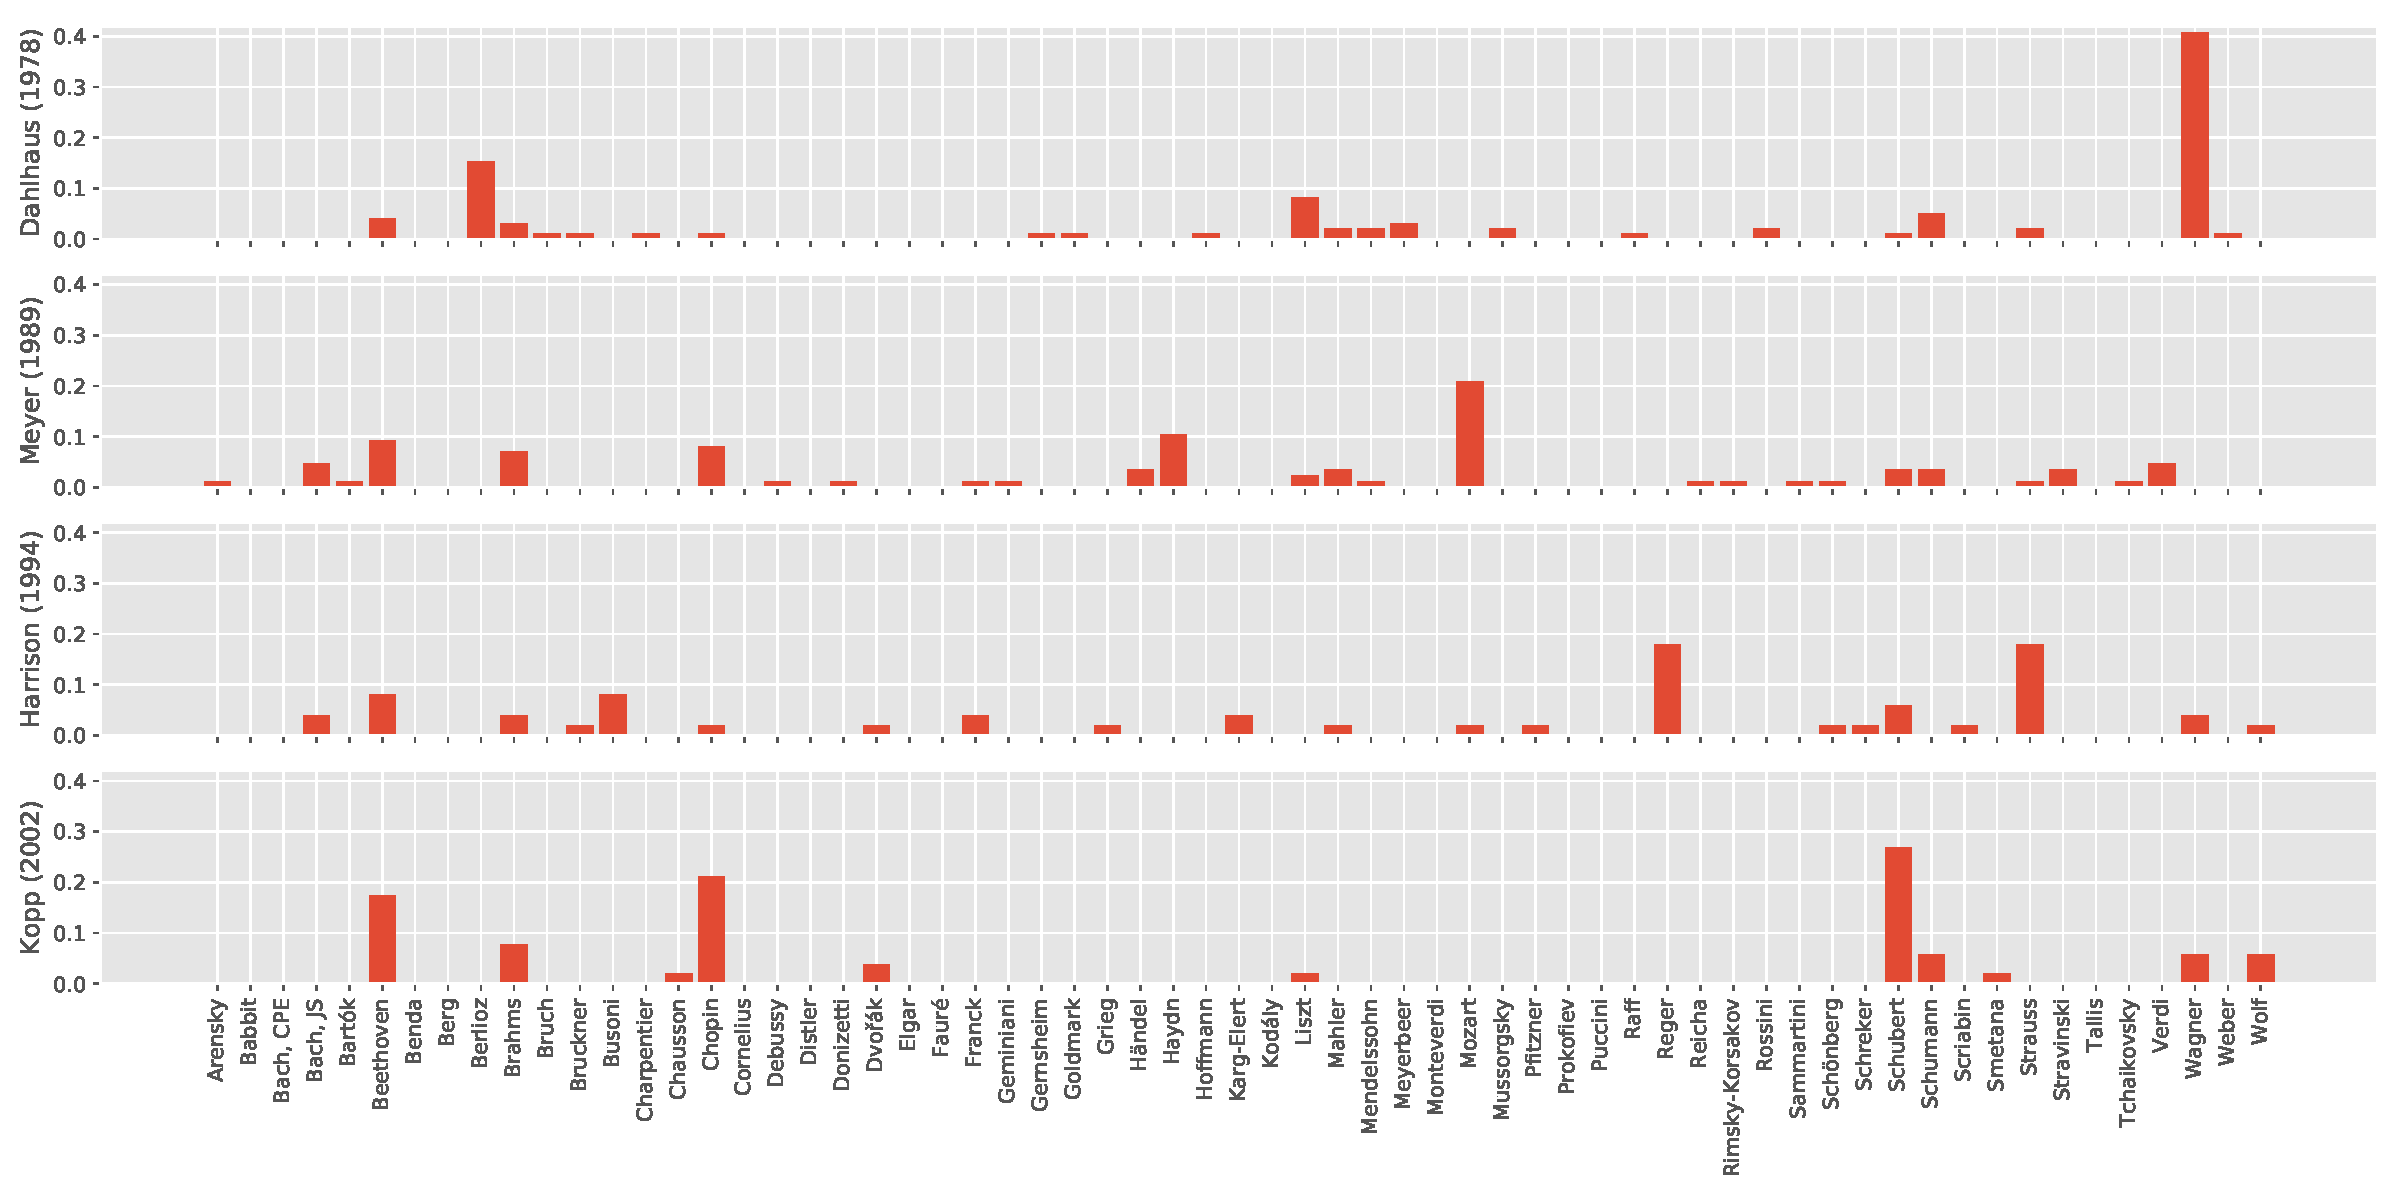
\includegraphics[width=.9\textwidth]{img/composer_counts.pdf}
    % \caption{}
    % \label{}
  \end{figure}
\end{frame}

\note[itemize]{
\item drawn conclusions may solely rely on different examples
\item implicit knowledge is inaccessible
}

\againframe<3>{cma}

\begin{frame}{\insertsectionhead}
  	\textbf{Definitions of Tonality}

   \begin{quote}
     ``the term is sometimes used as an equivalent for what Rousseau called
     a \emph{sistême musicale}, a rational and self-contained arrangement of musical phenomena''\\
     % [\ldots]. While tonality \emph{qua} system constitutes a theoretical
     % (and thus imaginative) abstraction from actual music, it is often hypostatized in
     % musicological discourse, converted from a theoretical structure into a musical reality.''\\
     \emph{\hfill\parencite{Hyer2001}}
  \end{quote}
  \vspace{1em}
  \pause
  \begin{quote}
    ``the relations between musical elements, e.g. notes or chords in a corpus''\\
    \emph{\hfill\parencite{Moss2019a}}
   \end{quote}
  % \onslide<2->{
  % \large
  % \begin{center}
  %   computational modeling $\color{epflred}{\Longleftrightarrow}$ corpus studies
  % \end{center}
  % }
\end{frame}

\note[itemize]{
  \item I like a definition by Brian Hyer in \emph{The New Grove Dictionary of Music and Musicians}.
}

\againframe<4->{cma}

% \begin{frame}<1-5>[label=disciplines]{\insertsectionhead}
%   \begin{center}
%     \begin{tikzpicture}
%       \node [visible on=<2->] (MT) at (0,0) {Music Theory};
%       \note[item]<2->{Music theory is the overarching framework}
%
%       \node [visible on=<3->] (part) at (-3,-4) {particular};
%       \draw[<->, >=stealth, line width=2, epfldark,visible on=<3->] (MT) -- (part) node [midway, sloped, above, epfldark] {Music Analysis};
%       \note[item]<3->{Music analysis looks at individual pieces, the particular}
%
%       \node [visible on=<4->] (gen) at (3, -4) {general};
%       \draw[<->, >=stealth, line width=2,  epfldark,visible on=<4->] (MT) -- (gen) node [midway, sloped, above, epfldark] {Corpus Studies};
%       \note[item]<4->{Corpus studies look at entire repertoires, aiming at describing the general.}
%
%       \draw[<->, >=stealth, line width=2, visible on=<5->] (part) -- (gen) node [visible on=<5->,align=center, midway,below] {Computational\\ Music Analysis}; % (CMA) at (0,-2.5)
%
%       \note[item]<5->{The mediating device are (formal) models. This is where my main research focus lies.}
%
%       \draw[<->, >=stealth, epflred, line width=2, visible on=<{6,8-}>] (MT) -- (gen);
%       \draw[<->, >=stealth, epflred, line width=2, visible on=<7->] (part) -- (gen);
%       \draw[<->, >=stealth, epflred, line width=2, visible on=<9>] (part) -- (MT);
%
%     \end{tikzpicture}
%   \end{center}
% \end{frame}
%
% \note[itemize]{
% \item Sampling bias can be addressed with Corpus Studies.
% \item Larger and common data
% \item instead of choosing suitable samples
% }

% \section{\thesection.~Understanding Chord Distributions}

% \againframe<5-6>{disciplines}

\begin{frame}{\insertsectionhead}
  \begin{enumerate}[\color{epflred}1.]
    \item<1-> \textbf{Corpus creation}\\ \citet{Neuwirth2018}.~\citetitle{Neuwirth2018}.
    \item<2-> \textbf{Corpus analysis}\\\citet{Moss2019b}.~\citetitle{Moss2019b}.
    \item<3-> \textbf{Corpus expansion}\\ \citet{Moss2019a}.~\citetitle{Moss2019a} (Diss.).
    % \item \emph{Distant Listening} project (2020--2024)
    % \item Mozart Sonatas (in preparation)
    % \item 24 other composers in preparation (16th--20th c.)
  \end{enumerate}
\end{frame}

\begin{frame}{\insertsectionhead}
  19th-century corpora (9 composers, 289 pieces)
  \begin{columns}
    \begin{column}{.4\linewidth}
      \begin{itemize}
        \item Beethoven: String quartets
        \item Schubert: \emph{Winterreise}
        \item Chopin: Mazurkas
        \item Liszt: \emph{Années de pèlerinage}
        \item Dvorák: \emph{Silhouettes}
        \item Grieg: \emph{Lyrical pieces}
        \item Tchaikovsky: \emph{Seasons}
        \item Debussy: \emph{Suite bergamasque}
        \item Medtner: \emph{Fairy tales}
      \end{itemize}
    \end{column}
    \pause
    \begin{column}{.6\linewidth}
      \begin{figure}
        \centering
        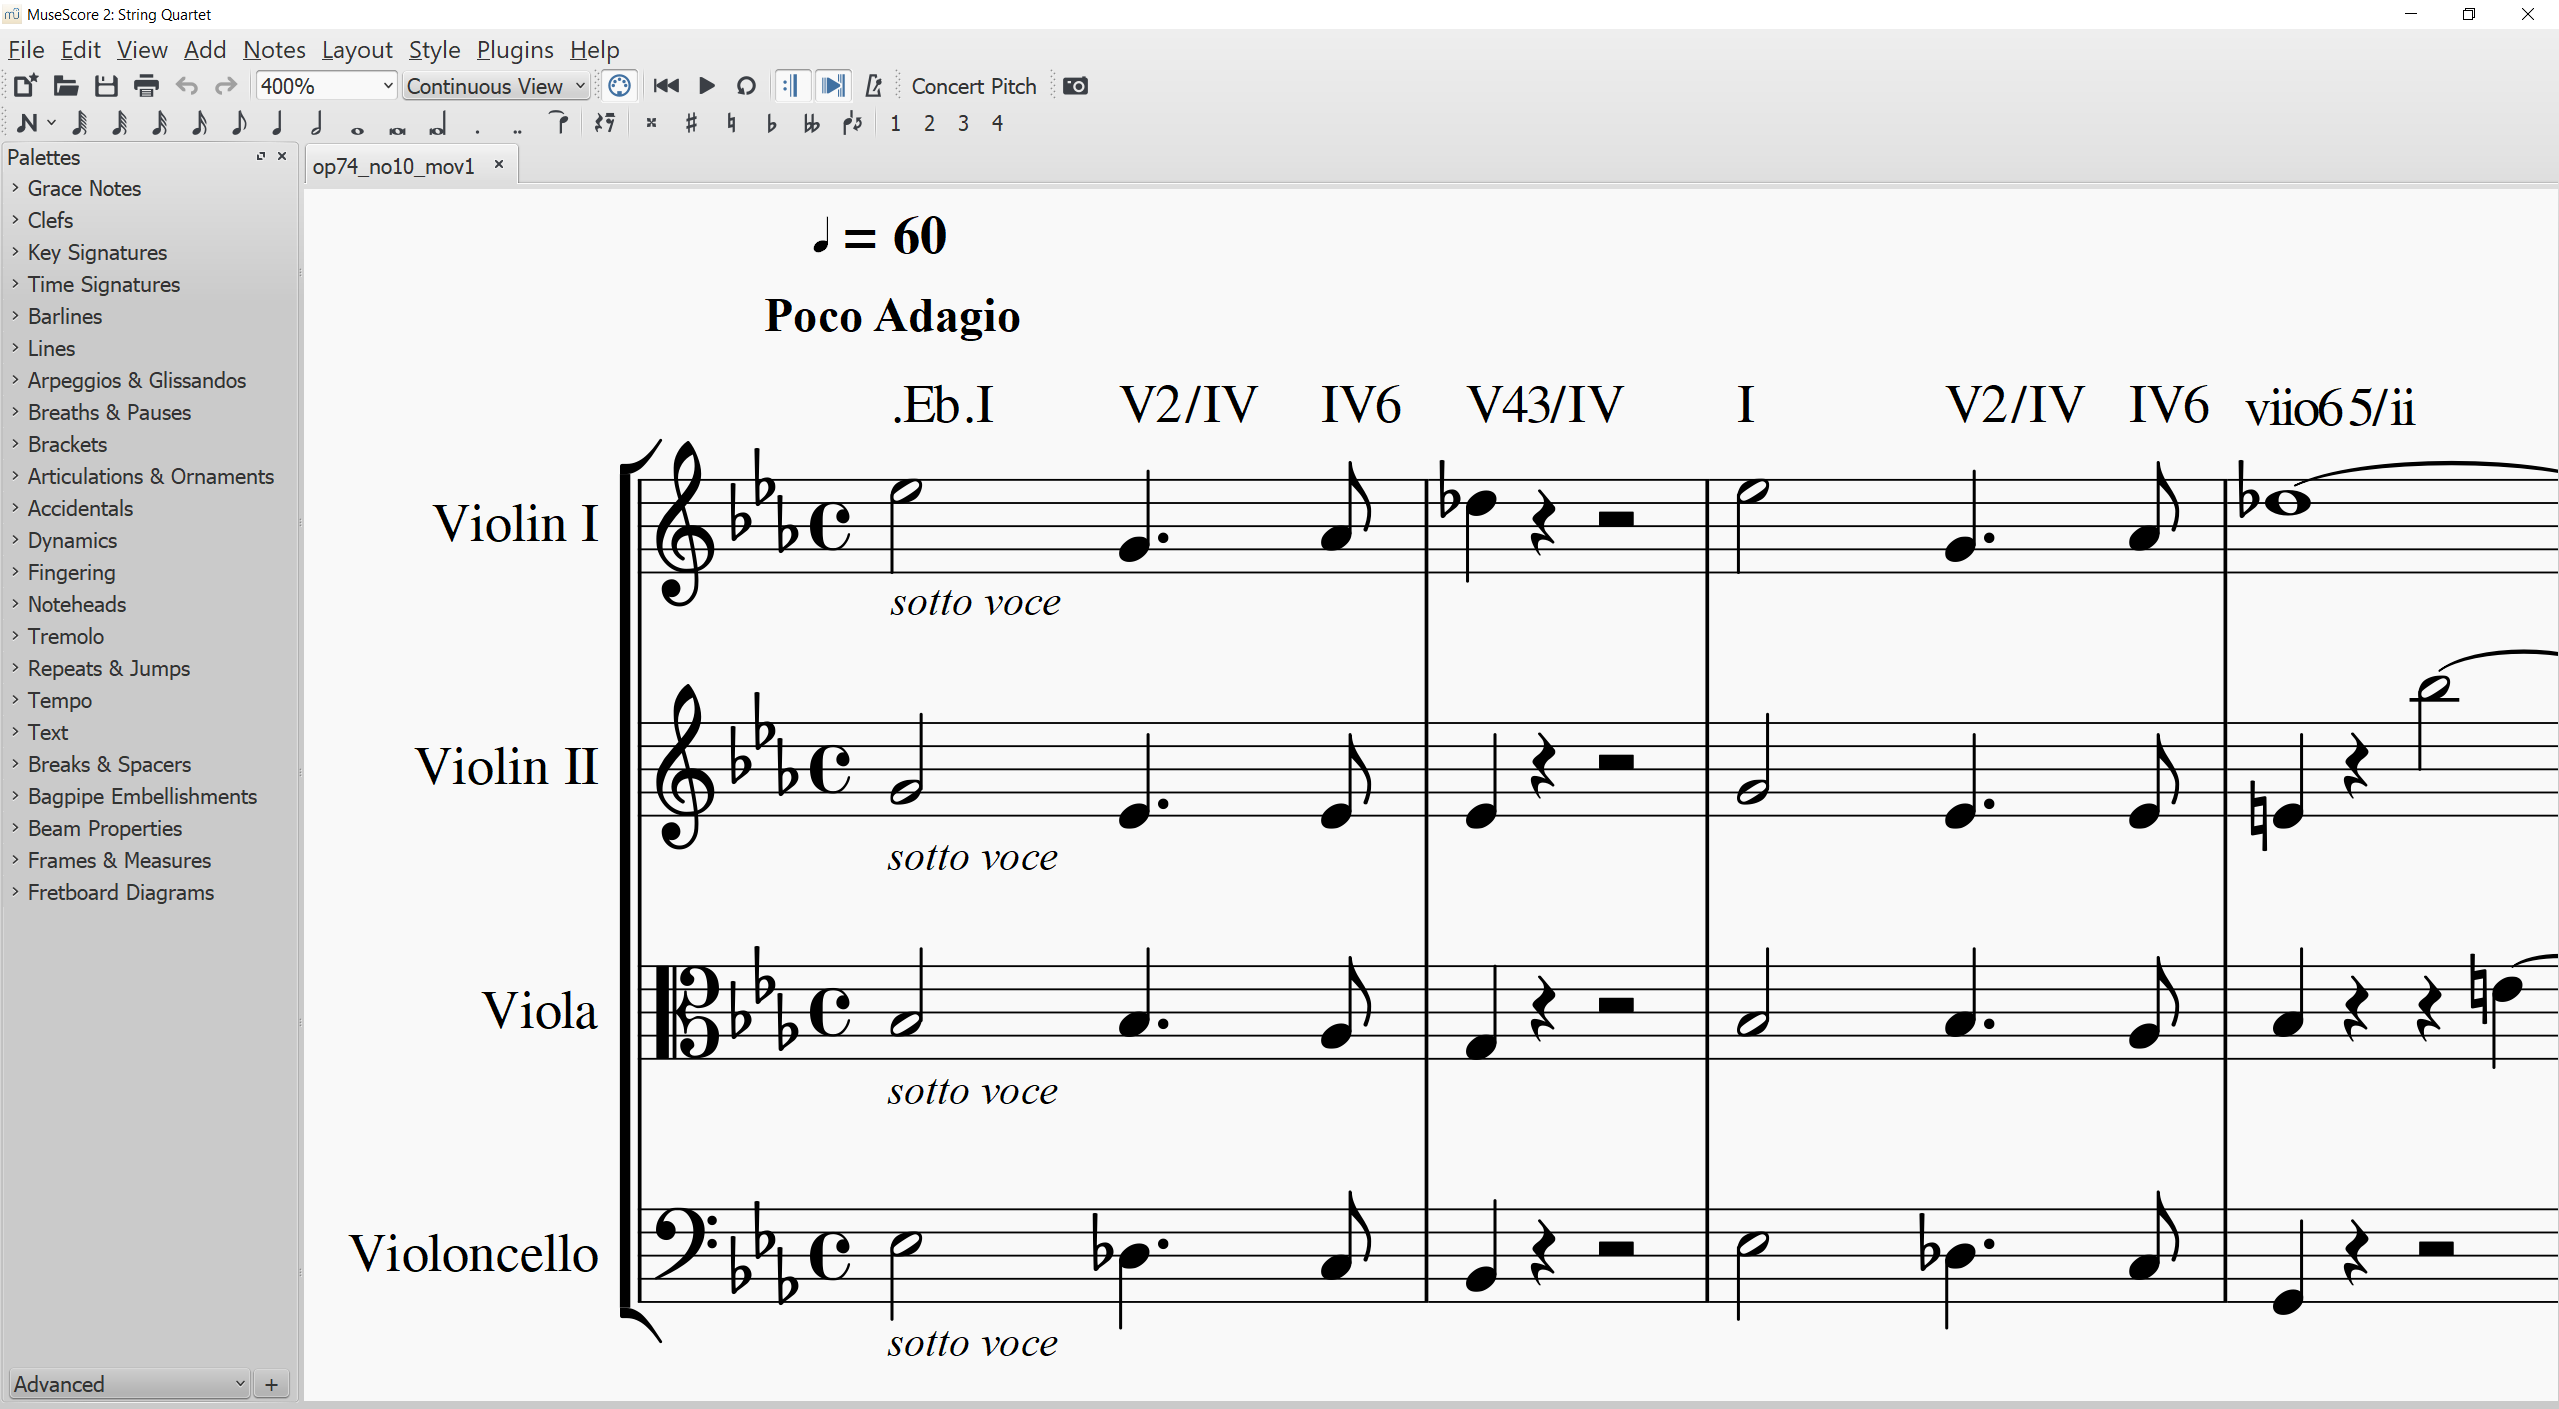
\includegraphics[width=\textwidth,height=.8\textheight,keepaspectratio]{img/musescore_screenshot.png}
        \caption{Chord annotation via \emph{MuseScore}.}
        \label{}
      \end{figure}
    \end{column}
  \end{columns}


\end{frame}

\begin{frame}<1-7>[label=corpus_pipeline]{\insertsectionhead}
  \onslide<1->{The corpus research pipeline}

  \resizebox{\textwidth}{!}{
  \centering
  \tikzstyle{my_arrow} = [->,>=stealth,shorten >= .5em, shorten <= .5em, line width=2pt]
  \begin{tikzpicture}
    \draw [visible on=<2->] (0,0) node (score) {
\includegraphics[height=1.5cm]{img/score.png}};

    \draw [visible on=<3->] (3,0) node (file) {
\includegraphics[height=1.5cm]{img/xml.png}};
    \draw [my_arrow,visible on=<3->] (score) -- (file) node [above,midway] {encoding};

    \draw [visible on=<4->] (6.5,3) node (expert) {
\includegraphics[height=1.5cm]{img/expert.png}};
    \draw [my_arrow,epflred,visible on=<4-7>] (expert) -- (file) node [midway,above left] {\color{epfldark}{analysis}};
    \draw [my_arrow,epflred!30,visible on=<8->] (expert) -- (file) node [midway,above left] {\color{epfldark!30}{analysis}};

    \draw [visible on=<5-7>] (7,0) node (vec) {\footnotesize$x=\begin{bmatrix}I\\V7\\ii6\\V7/IV\\\sharp viio\\\vdots\end{bmatrix}$};
    \draw [visible on=<8->] (7,0) node (vec) {\footnotesize$x=\begin{bmatrix}B\flat\\G\\A\\G\\C\sharp\\\vdots\end{bmatrix}$};
    \draw [my_arrow,visible on=<5->] (file) -- (vec) node [above,midway] {extraction};

    \draw [visible on=<6-7>] (12,0) node (dist) {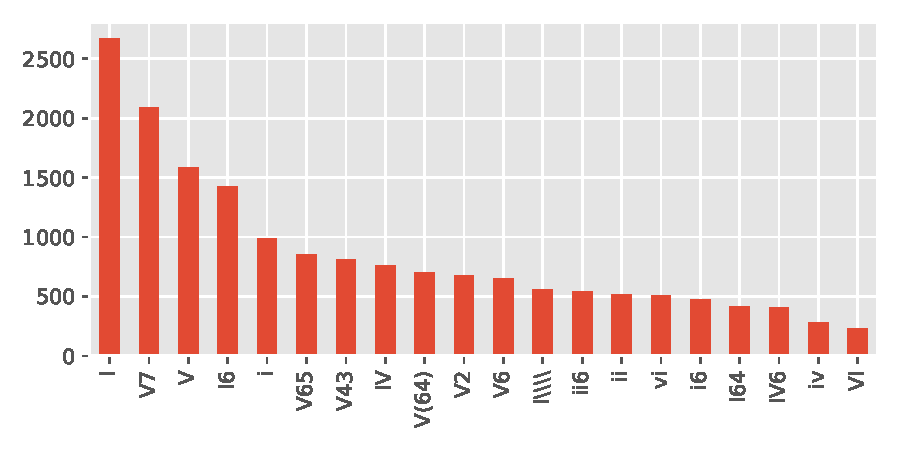
\includegraphics[width=4cm]{img/chord_stats.pdf}};
    \draw [visible on=<8->] (12,0) node (dist) {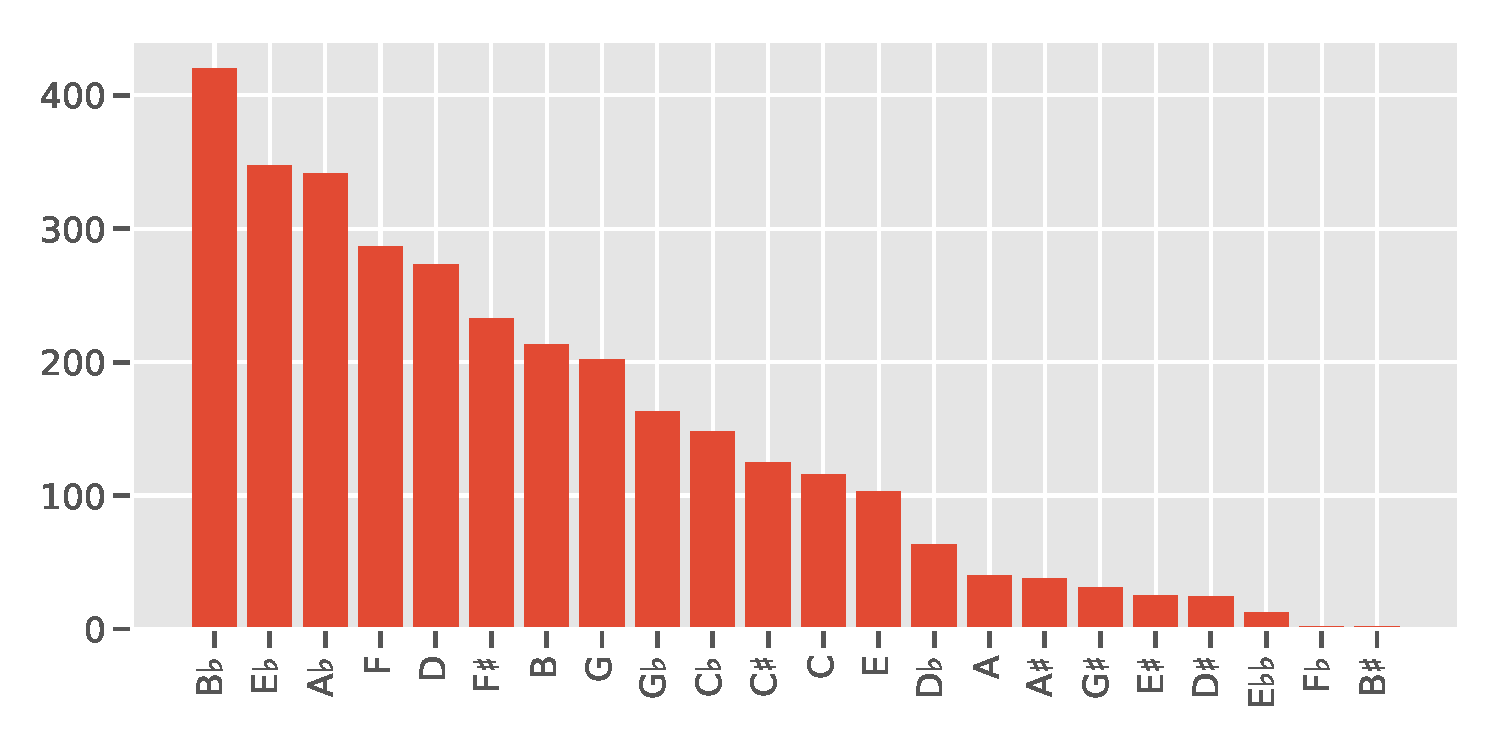
\includegraphics[width=4cm]{img/tpc_dists_sorted.pdf}};
    \draw [my_arrow,visible on=<6->] (vec) -- (dist) node [above, midway] {statistics};

    \draw [my_arrow,visible on=<7->, epflred] (expert) -- (dist) node [above right, midway] {\color{epfldark}{interpretation}};

  \end{tikzpicture}
  }
\end{frame}

\begin{frame}{\insertsectionhead}
  A fundamental distinction in corpus research:

  \begin{itemize}
    \item \alert{all chords} that occur in a corpus $\mathcal C$ (chord tokens), e.g.
  \end{itemize}
  \begin{align*}
    T_{\mathcal C} = \{\, I : 12,\, V7 : 6,\, V : 5,\, ii : 5,\, IV : 4,\, I6 : 2,\, III : 1,\, viio7 : 1\,\}
  \end{align*}
  \pause
  \begin{itemize}
    \item \alert{all unique chords} that occur in a corpus $\mathcal C$ (chord types), e.g.
  \end{itemize}
  \begin{align*}
    t_{\mathcal C} = \{\, I, V7, V, ii, IV, I6, III, viio7 \,\}
  \end{align*}
\end{frame}


\begin{frame}{\insertsectionhead}

  \begin{columns}
    \begin{column}{.7\textwidth}
\def\firstcircle{(0,0) circle (1.2cm)}
\def\secondcircle{(60:2cm) circle (2cm)}
\def\thirdcircle{(120:2cm) circle (1.5cm)}
\tikzstyle{corpus}=[line width=0mm,epflred,fill, opacity=0]
\begin{center}
\begin{tikzpicture}
  \draw[corpus,fill opacity=0.2, visible on=<1->]
    \firstcircle node[black,below,opacity=1] {$\mathcal C_1$};
    %
    \draw[corpus,fill opacity=0.4, visible on=<2->]
    \secondcircle node[black,right,opacity=1] {$\mathcal C_2$};
    %
    \draw[corpus,fill opacity=0.6, visible on=<3->]
    \thirdcircle node[black,left,opacity=1] {$\mathcal C_3$};
    %
    \draw [thick,decorate,decoration={brace,amplitude=10pt},visible on=<4->] (-3,-1.5) -- (-3,4) node [midway, left, xshift=-5mm,align=center]  {Vocabulary:\\3,185 unique chords\\(75,380 chords in total)}; % \\3185 types
    \node [align=center, visible on=<5->] (core) at (3,-1) {Core:\\43 unique chords}; %  $\mathbb C$\\43 types
    \node (intersection) at (-.45,.85) {};
    \draw[->,>=stealth,thick, visible on=<5->] (core) -- (intersection);
\end{tikzpicture}
\end{center}
\end{column}
%
\begin{column}{.3\textwidth}
  \onslide<6->{
\begin{align*}
  \frac{|Core|}{|Vocabulary|} \approx 1.35\text{\%}
\end{align*}}
\end{column}
\end{columns}
\end{frame}

\begin{frame}{\insertsectionhead}
\onslide<1->{
\small
  \begin{align*}
   \text{Core} = \{\;
      & \mathsf{I},\, \mathsf{I6},\, \mathsf{I64},\, \mathsf{i},\, \mathsf{i6},\, \mathsf{i64},\, \nonumber\\
      & \mathsf{ii},\, \mathsf{ii6},\, \mathsf{ii7},\, \mathsf{ii65},\, \mathsf{iio},\, \mathsf{ii\emptyset 7},\, \mathsf{ii\emptyset 43},\, \mathsf{ii\emptyset 2},\, \nonumber\\
      & \mathsf{iii},\, \mathsf{iii6},\, \mathsf{III},\, \nonumber\\
      & \mathsf{IV},\, \mathsf{IV6},\, \mathsf{iv},\, \mathsf{iv64},\, \nonumber\\
      & \mathsf{V},\, \mathsf{V6},\, \mathsf{V64},\, \mathsf{V7},\, \mathsf{V7(4)},\, \mathsf{V65},\, \mathsf{V43},\, \mathsf{V2},\, \nonumber\\
      & \mathsf{vi},\, \mathsf{vi6},\, \mathsf{VI},\, \mathsf{VI6},\, \nonumber\\
      & \mathsf{viio6},\, \mathsf{\sharp viio6},\, \mathsf{\sharp viio43},\, \nonumber\\
      & \mathsf{V65/III},\, \mathsf{V7/IV},\, \mathsf{V2/IV},\, \mathsf{V65/V},\, \mathsf{V43/V},\, \mathsf{V2/V},\, \mathsf{\sharp viio7/vi} \;\}
      \label{eq:core}
  \end{align*}}

  \onslide<2->{
  \normalsize
  Between 45 and 74\% of all chords are core chords!
  }
\end{frame}
%
\note[itemize]{

\item this collection consists of the \alert{typical cases} one would find in a harmony text book
\item consequently, textbook harmonic analysis takes only ~1\% of all chords into account
\item How can this be justified?
}

\begin{frame}{\insertsectionhead}
  $\Rightarrow$ What affects the frequency of chords?
\end{frame}

\begin{frame}{\insertsectionhead}
  \begin{columns}
    \begin{column}{.53\linewidth}
      \textbf{Zipf's law}~\citep{Zipf1949}

      The relation between \alert{frequency}~$f$ and \alert{rank}~$r$ (1st, 2nd,\ldots, $n$th) resembles a power law:
      \begin{align*}
        f(r) \approx \frac{\alpha}{(\beta + r)^\gamma}
      \end{align*}
    \end{column}\hfill
    \pause
    \begin{column}{.47\linewidth}
      \begin{figure}
        \centering
        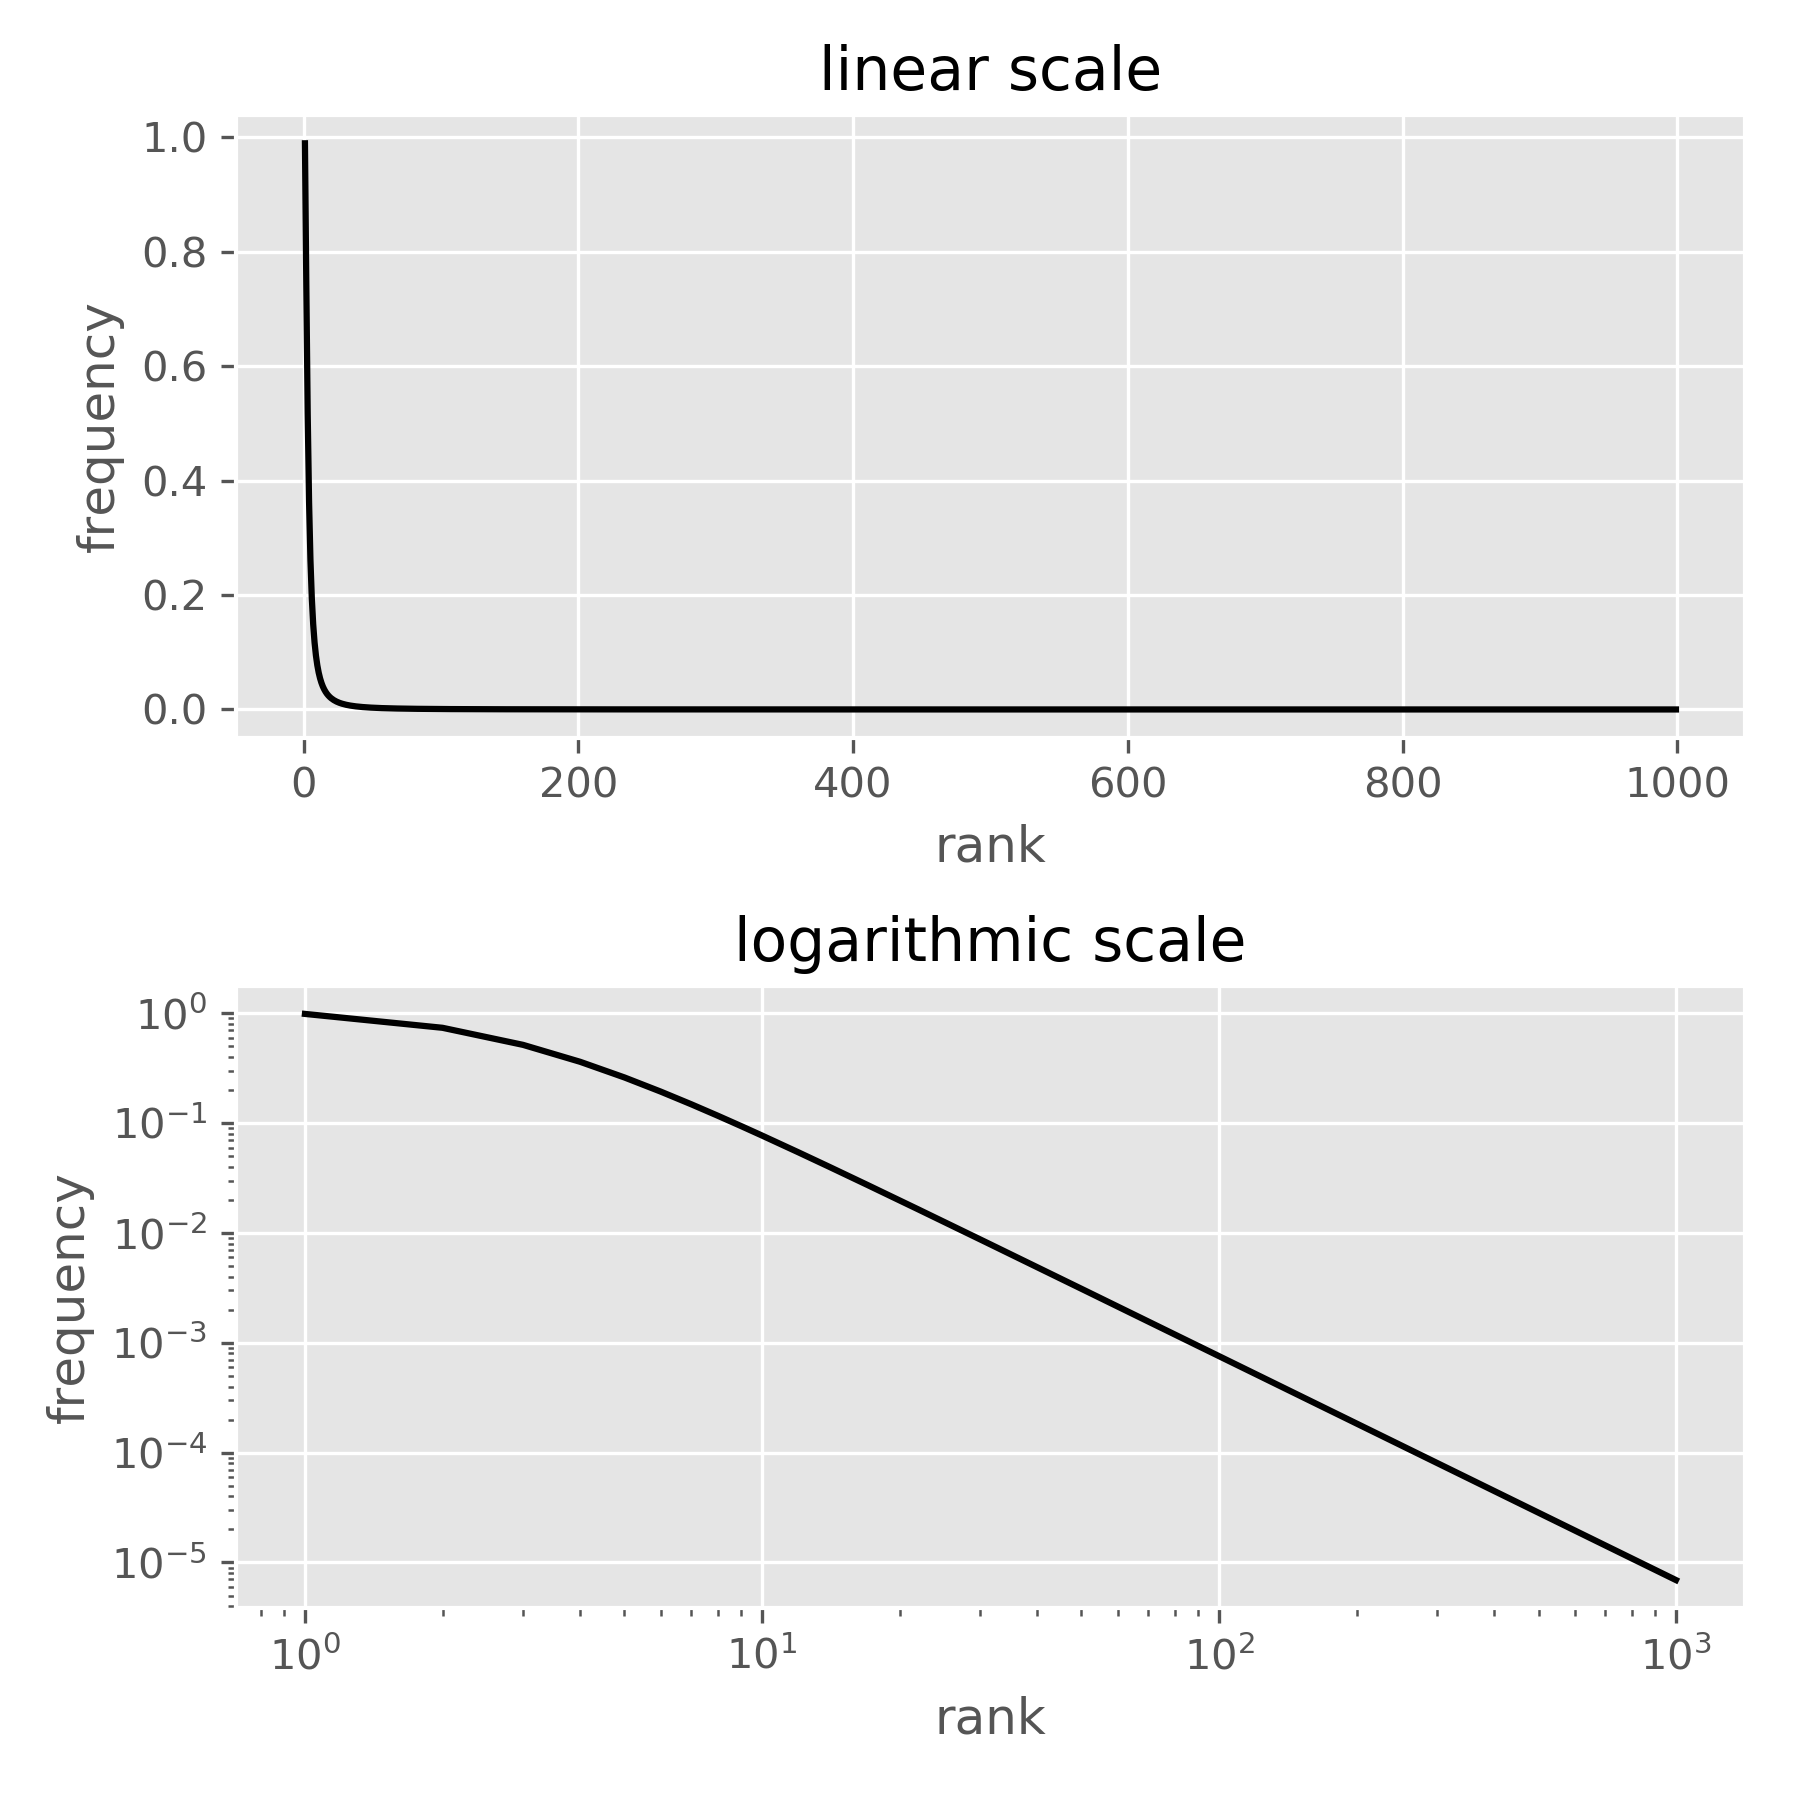
\includegraphics[width=\textwidth]{img/zipf_model.png}
      % \caption{Zipf curve with arbitrary parameters}
      \end{figure}
    \end{column}
  \end{columns}
  % This relation is ubiquitous in linguistics and musicology \parencite{Rohrmeier2008,Piantadosi2014}. Do the annotated corpora \alert{conform} to this phenomenon?
\end{frame}

\begin{frame}{\insertsectionhead}
  \begin{figure}
    % \begin{subfigure}[c]{.6\linewidth}
      \centering
      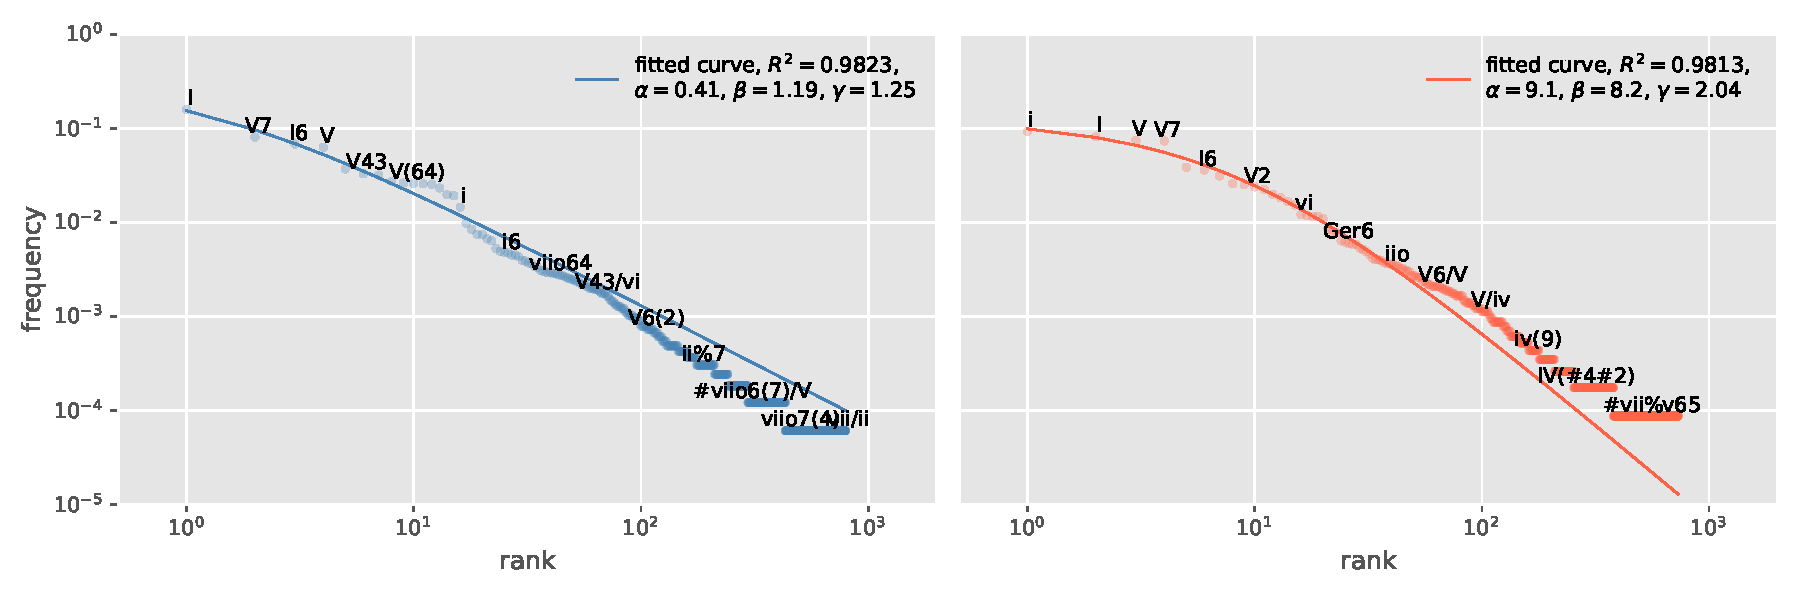
\includegraphics[width=\textwidth]{img/ABC_zipf_mandelbrot.pdf}
      \caption{Chord distribution in Beethoven's string quartets.}
    % \end{subfigure}\vfill
    % \begin{subfigure}[c]{.6\linewidth}
    %   \centering
    %   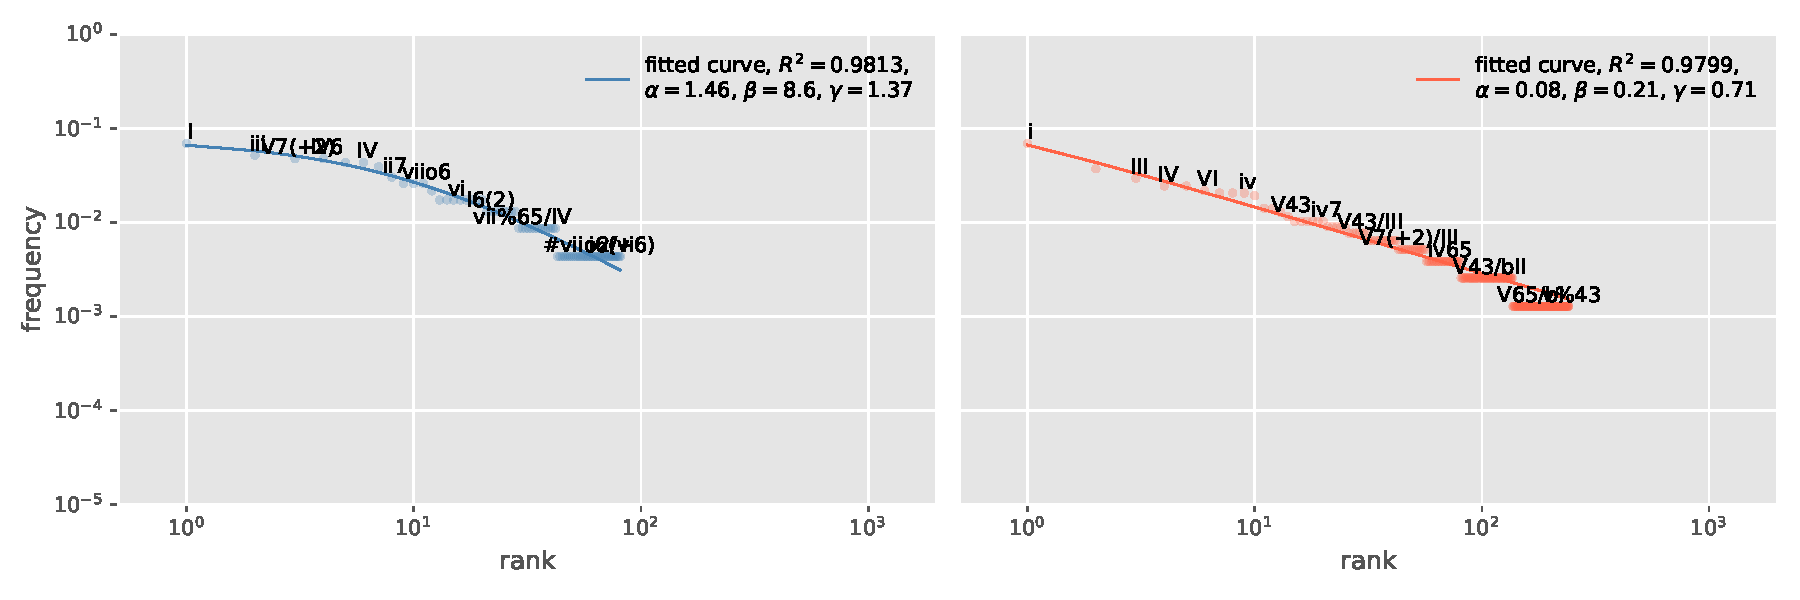
\includegraphics[width=\textwidth]{img/debussy_zipf_mandelbrot.pdf}
    %   \caption{Debussy's \emph{Suite bergamasque}.}
    % \end{subfigure}
  \end{figure}
\end{frame}

\begin{frame}{\insertsectionhead}
  \begin{enumerate}[\color{epflred}1.]
    \item<1-> Zipf's law is found in many domains (e.g. language, social networks, citations, \ldots)
    \item<2-> What is specific about tonal music?
    \item<3-> Many processes could explain this finding~\citep{Piantadosi2014}
    % \item<4-> More sophisticated models are needed
  \end{enumerate}
  \onslide<4->{$\Rightarrow$ Addressing these issues by closer inspecting \alert{deviations} from the model}
\end{frame}

\begin{frame}{\insertsectionhead}
  \begin{figure}
    \centering
    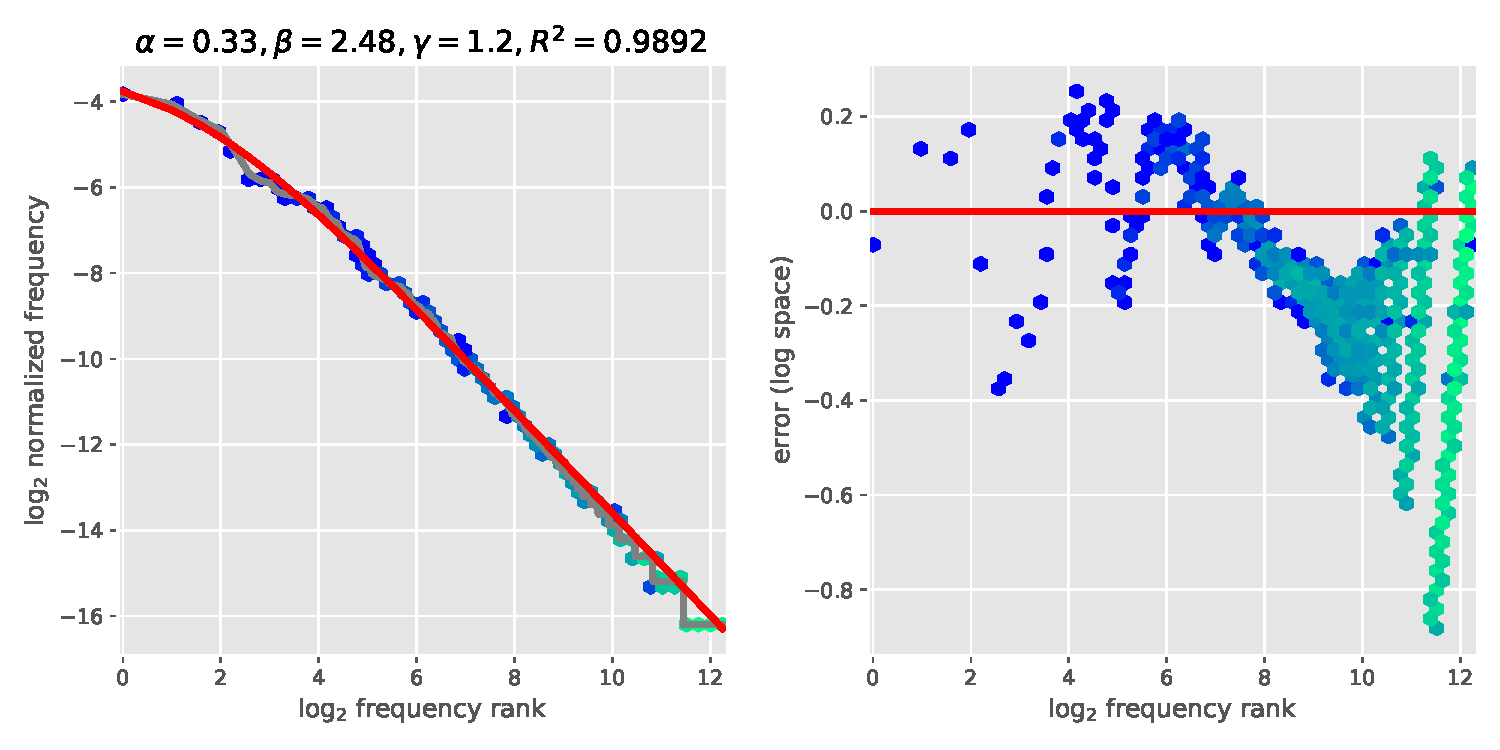
\includegraphics[width=.8\textwidth]{img/freqrank_disterror.pdf}
    \caption{Zipf-fit of chord distribution (left). Deviations from model (right).}
    \label{}
  \end{figure}
\end{frame}

\begin{frame}{\insertsectionhead}
  \begin{itemize}
    \item<1-> \alert{new insight}: systematic deviations from standard models of chord distributions
    \item<2-> development of more advanced models in future research
    \item<3-> impossible without the computational approach
  \end{itemize}

\end{frame}

% \begin{frame}{Summary and Prospects}
%   \begin{enumerate}[\color{epflred}1.]
%     \item \ldots
%     \item \ldots
%     \item \ldots
%     \label{}
%   \end{enumerate}
% \end{frame}

% \section{\thesection.~A Data-Driven History of Tonality}

% \againframe<{5,7}>{disciplines}

% \begin{frame}{\insertsectionhead}
%   Motivation / Questions
% \end{frame}

\againframe<7->{corpus_pipeline}

\subsection{1. Recovering the line of fifths}

\begin{frame}{\insertsectionhead}
    \onslide<3->{
    \begin{center}
    \resizebox{.75\textwidth}{!}{
      % colors for line of fifths
\definecolor{Gb}{HTML}{6d6dff}
\definecolor{Db}{HTML}{8585ff}
\definecolor{Ab}{HTML}{9d9dff}
\definecolor{Eb}{HTML}{b5b5ff}
\definecolor{Bb}{HTML}{cdcdff}
\definecolor{F}{HTML}{e5e5ff}
\definecolor{C}{HTML}{fffdfd}
\definecolor{G}{HTML}{ffe5e5}
\definecolor{D}{HTML}{ffcdcd}
\definecolor{A}{HTML}{ffb5b5}
\definecolor{E}{HTML}{ff9d9d}
\definecolor{B}{HTML}{ff8585}
\definecolor{Fs}{HTML}{ff6d6d}

% draw picture
\begin{tikzpicture}[scale=2]

\draw[latex-latex] (-3.5,0) -- (3.5,0) ; % line

% down ticks
\foreach \x/\label in  {-6/G$\flat$,
                         -5/D$\flat$,
                         -4/A$\flat$,
                         -3/E$\flat$,
                         -2/B$\flat$,
                         -1/F,
                         0/C,
                         1/G,
                         2/D,
                         3/A,
                         4/E,
                         5/B,
                         6/F$\sharp$}
\draw[shift={(\x/2,0)},color=black] (0pt,0pt) -- (0pt,-5pt) node[below] {\label};
% % up ticks
% \foreach \x in  {-6,...,6}
% \draw[shift={(\x/2,0)},color=black] (0pt,0pt) -- (0pt,5pt) node[above] {$\x$};

% draw circles
\foreach \x/\color in {-6/Gb,
                         -5/Db,
                         -4/Ab,
                         -3/Eb,
                         -2/Bb,
                         -1/F,
                         0/C,
                         1/G,
                         2/D,
                         3/A,
                         4/E,
                         5/B,
                         6/Fs}
  \node [circle, fill=\color,scale=1.5, draw=black] (\x) at (\x/2,0) {};

\end{tikzpicture}
}
    \end{center}
  }

  \begin{figure}
    \onslide<2->{
    \begin{subfigure}[c]{.48\linewidth}
      \centering
      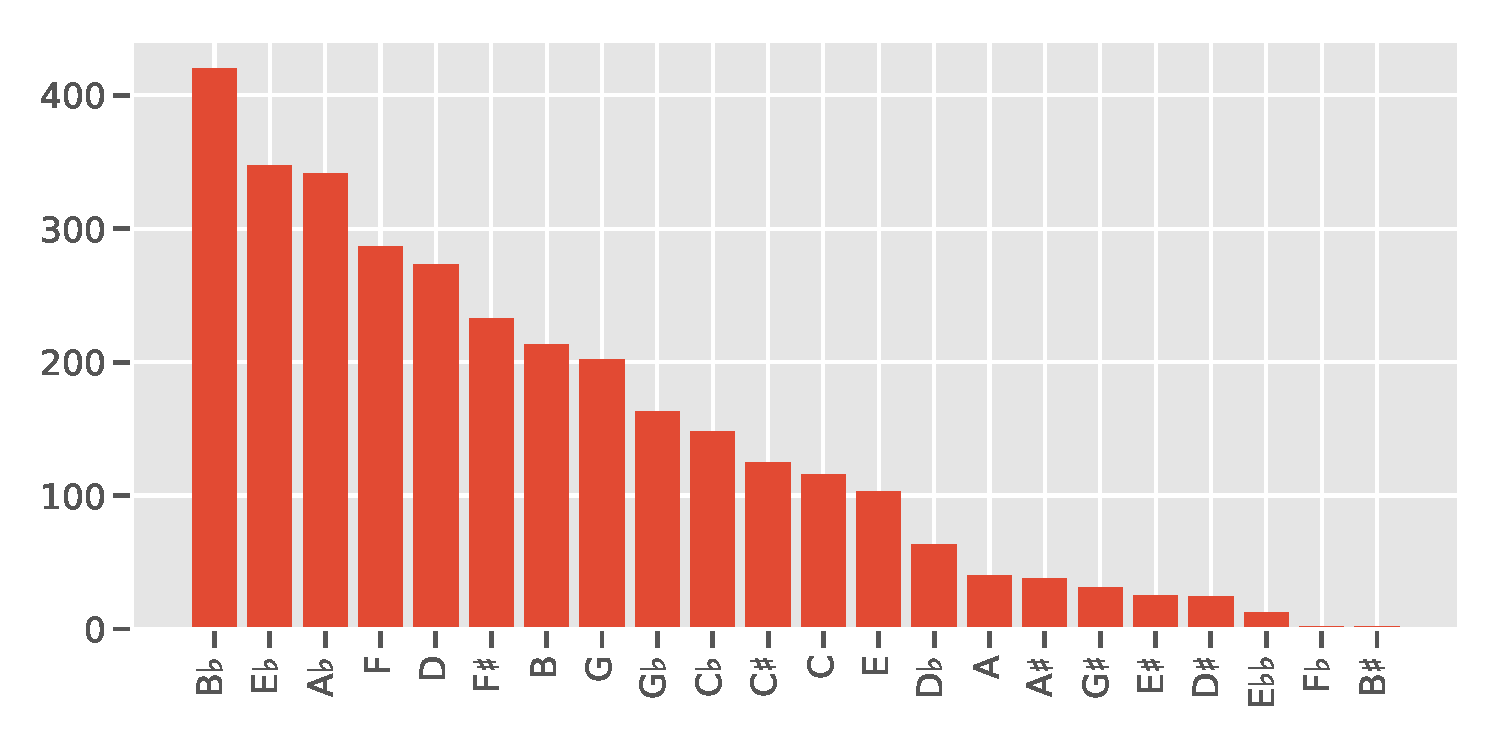
\includegraphics[width=\textwidth]{img/tpc_dists_sorted.pdf}
      \subcaption{Ranked note frequencies.}
    \end{subfigure}
    }
    \hfill
    \onslide<4->{
    \begin{subfigure}[c]{.48\linewidth}
      \centering
      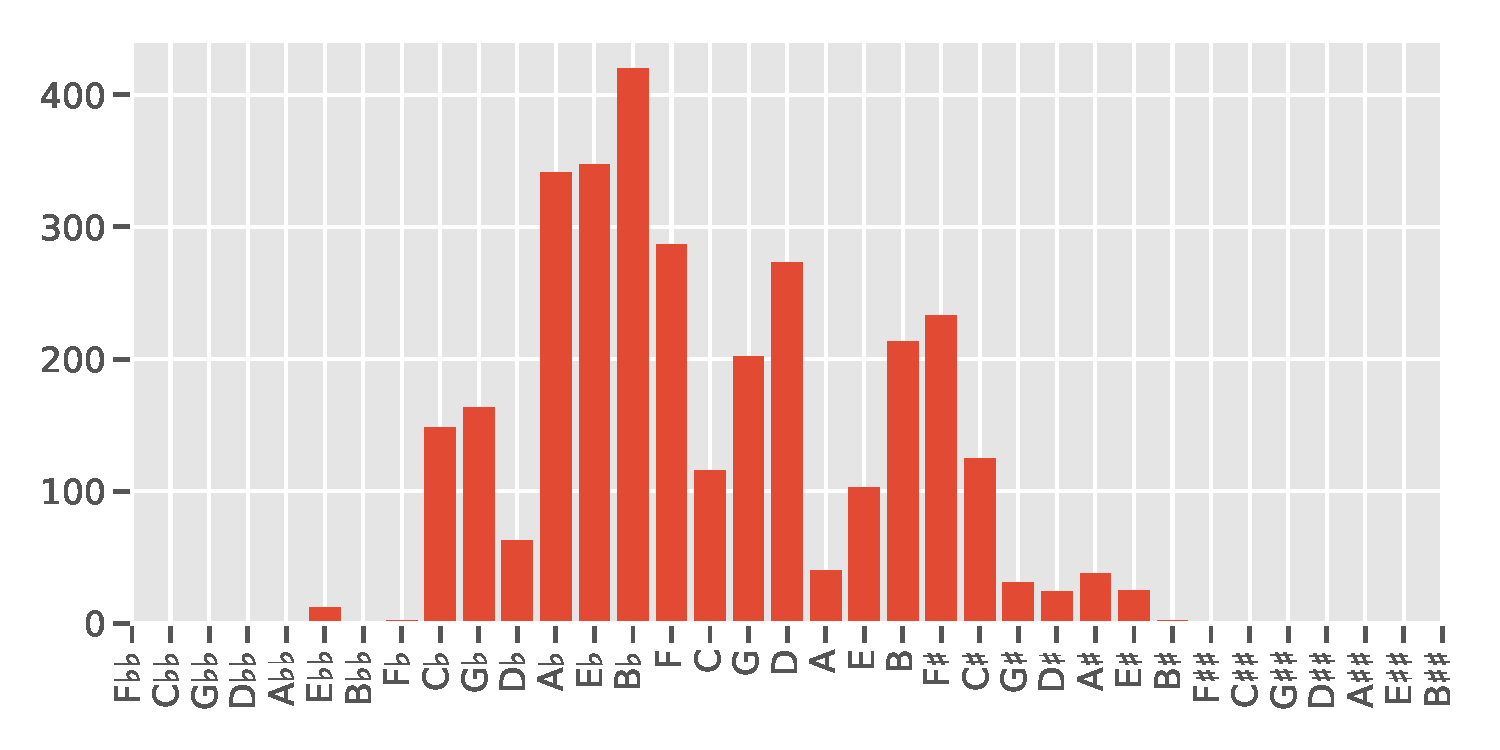
\includegraphics[width=\textwidth]{img/tpc_dists.pdf}
      \subcaption{Note frequencies on line of fifths.}
    \end{subfigure}
    }
    \caption{F. Schubert, \emph{Impromptu}, op.~90/2 in E$\flat$~major.}
    \label{}
  \end{figure}
\end{frame}

\note[itemize]{
  \item Using Music Theory: arranging on LoF shows structure
  \item define fifth width
  \item FW >= 7: chromaticism; FW >= 12: enharmonicism
}

\begin{frame}{\insertsectionhead}

  Corpus studies allow us to
  \begin{itemize}
    \item widen the \alert{scope} to entire collections of pieces
    \item empirically \alert{test} the validity of music-theoretical concepts
  \end{itemize}

  \pause

  $\Rightarrow$ Is the line of fifths \emph{really} a \alert{relevant structure} for pitch-class distributions?

  \pause

  \begin{enumerate}[\color{epflred}1.]
    \item Gather a large corpus.
    \item Transform pieces to pitch-class distributions.
    \item Apply \emph{dimensionality reduction} to uncover underlying structures.
  \end{enumerate}
\end{frame}

\begin{frame}{\insertsectionhead}

  \begin{columns}
    \begin{column}{.3\textwidth}
      % Sources
      % \begin{itemize}
      %   \item existing published \& accessible data
      %   \item web search
      %   \item transcription
      % \end{itemize}
      % Dataset \citep{Moss2020}
      The corpus:
      \begin{itemize}
        \item 2,012 pieces
        \item 75 composers
        \item approx. 600 years
      \end{itemize}
    \end{column}
    %
    \begin{column}{.7\textwidth}
      \begin{figure}
        \centering
        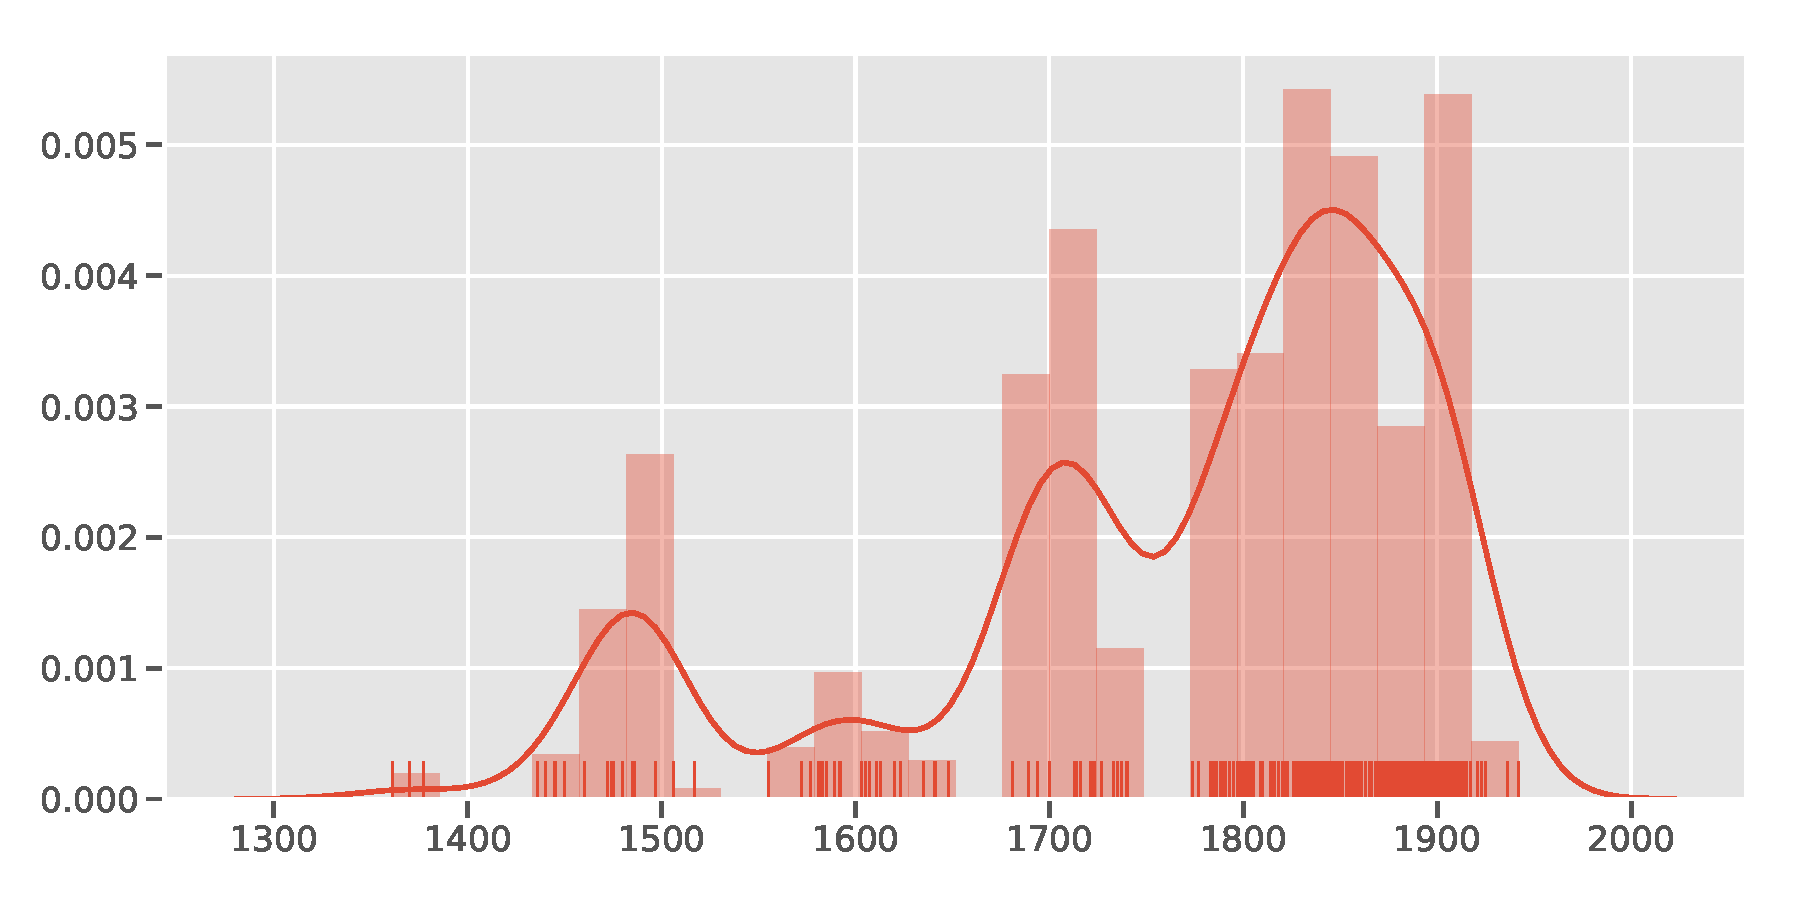
\includegraphics[width=\textwidth]{img/piece_dist.pdf}
        \caption{Historical distribution of the corpus.}
        \label{}
      \end{figure}
    \end{column}
  \end{columns}
\end{frame}

\begin{frame}{\insertsectionhead}
  \begin{figure}
  \captionsetup[subfigure]{justification=centering}
    \onslide<2->{
      \begin{subfigure}[t]{.3\textwidth}
        \centering
        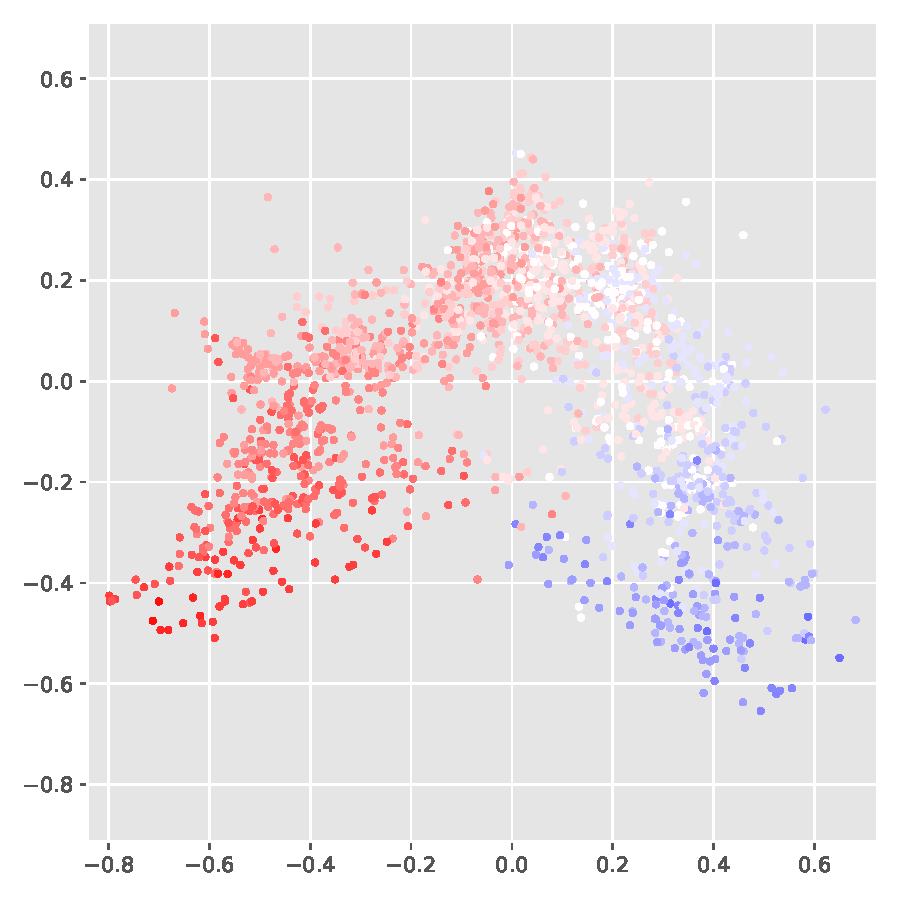
\includegraphics[width=\linewidth]{img/dim_reduct_Isomap.pdf}
        \subcaption*{Isomap.}
      \end{subfigure}
    }
    \hfill
    \onslide<1->{
      \begin{subfigure}[t]{.3\textwidth}
        \centering
        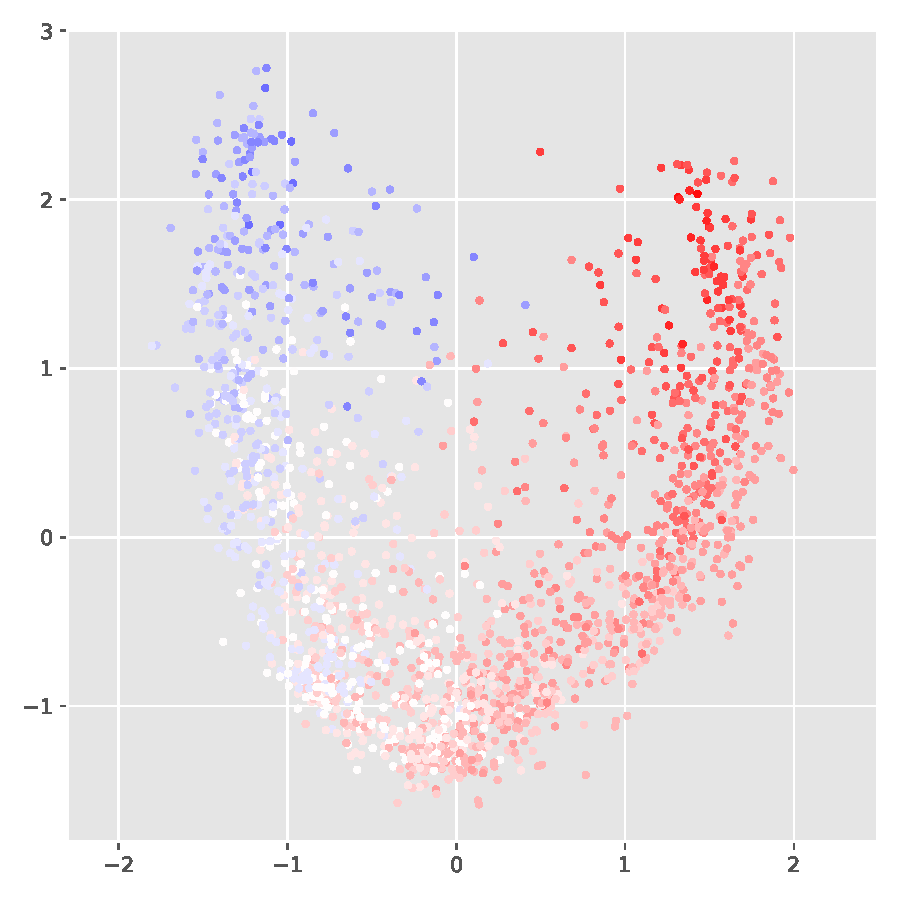
\includegraphics[width=\linewidth]{img/dim_reduct_PCA.pdf}
        \subcaption*{Principal Component Analysis.}
      \end{subfigure}
    }
    \hfill
    \onslide<2->{
    \begin{subfigure}[t]{.3\textwidth}
      \centering
      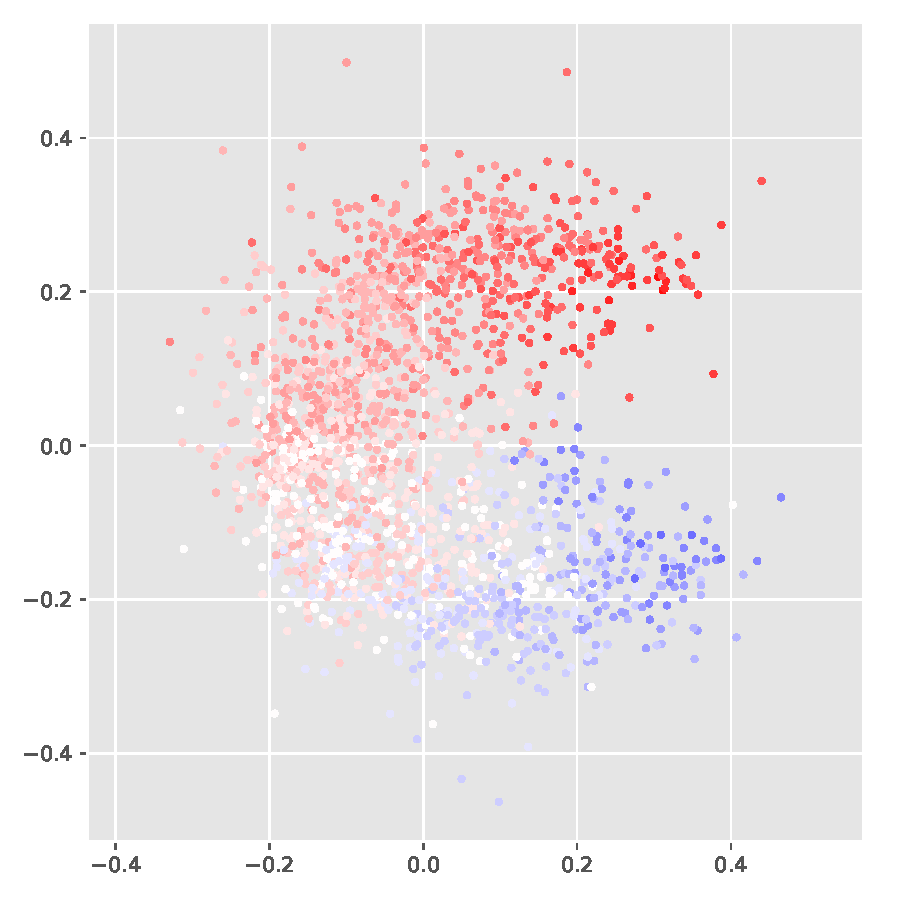
\includegraphics[width=\linewidth]{img/dim_reduct_MDS.pdf}
      \subcaption*{Multi-Dimensional Scaling.}
    \end{subfigure}
    }
    \caption{Dimensionality reduction of tonal space.}
    \label{}
  \end{figure}

  \onslide<1->{
    \begin{center}
    \resizebox{.75\textwidth}{!}{
      % colors for line of fifths
\definecolor{Gb}{HTML}{6d6dff}
\definecolor{Db}{HTML}{8585ff}
\definecolor{Ab}{HTML}{9d9dff}
\definecolor{Eb}{HTML}{b5b5ff}
\definecolor{Bb}{HTML}{cdcdff}
\definecolor{F}{HTML}{e5e5ff}
\definecolor{C}{HTML}{fffdfd}
\definecolor{G}{HTML}{ffe5e5}
\definecolor{D}{HTML}{ffcdcd}
\definecolor{A}{HTML}{ffb5b5}
\definecolor{E}{HTML}{ff9d9d}
\definecolor{B}{HTML}{ff8585}
\definecolor{Fs}{HTML}{ff6d6d}

% draw picture
\begin{tikzpicture}[scale=2]

\draw[latex-latex] (-3.5,0) -- (3.5,0) ; % line

% down ticks
\foreach \x/\label in  {-6/G$\flat$,
                         -5/D$\flat$,
                         -4/A$\flat$,
                         -3/E$\flat$,
                         -2/B$\flat$,
                         -1/F,
                         0/C,
                         1/G,
                         2/D,
                         3/A,
                         4/E,
                         5/B,
                         6/F$\sharp$}
\draw[shift={(\x/2,0)},color=black] (0pt,0pt) -- (0pt,-5pt) node[below] {\label};
% % up ticks
% \foreach \x in  {-6,...,6}
% \draw[shift={(\x/2,0)},color=black] (0pt,0pt) -- (0pt,5pt) node[above] {$\x$};

% draw circles
\foreach \x/\color in {-6/Gb,
                         -5/Db,
                         -4/Ab,
                         -3/Eb,
                         -2/Bb,
                         -1/F,
                         0/C,
                         1/G,
                         2/D,
                         3/A,
                         4/E,
                         5/B,
                         6/Fs}
  \node [circle, fill=\color,scale=1.5, draw=black] (\x) at (\x/2,0) {};

\end{tikzpicture}
}
    \end{center}
  }

\end{frame}

\note[itemize]{
  \item Uncovering underlying spaces: dimensionality reduction
  \item Empirical validation of MT conception of tonal space
  \item comparison of different methods shows that result is robust
}

\begin{frame}{\insertsectionhead}

  \begin{enumerate}[\color{epflred}1.]
    \item<1-> \alert{Historical changes} in the distributions of pitch classes?
    \item<2-> Important \alert{transitions} in the way composers write music on a large scale?
    \item<3-> Observe the \alert{expansion} of tonal material on line of fifths.
  \end{enumerate}

\end{frame}

\begin{frame}{\insertsectionhead}
  \begin{figure}
    \centering
    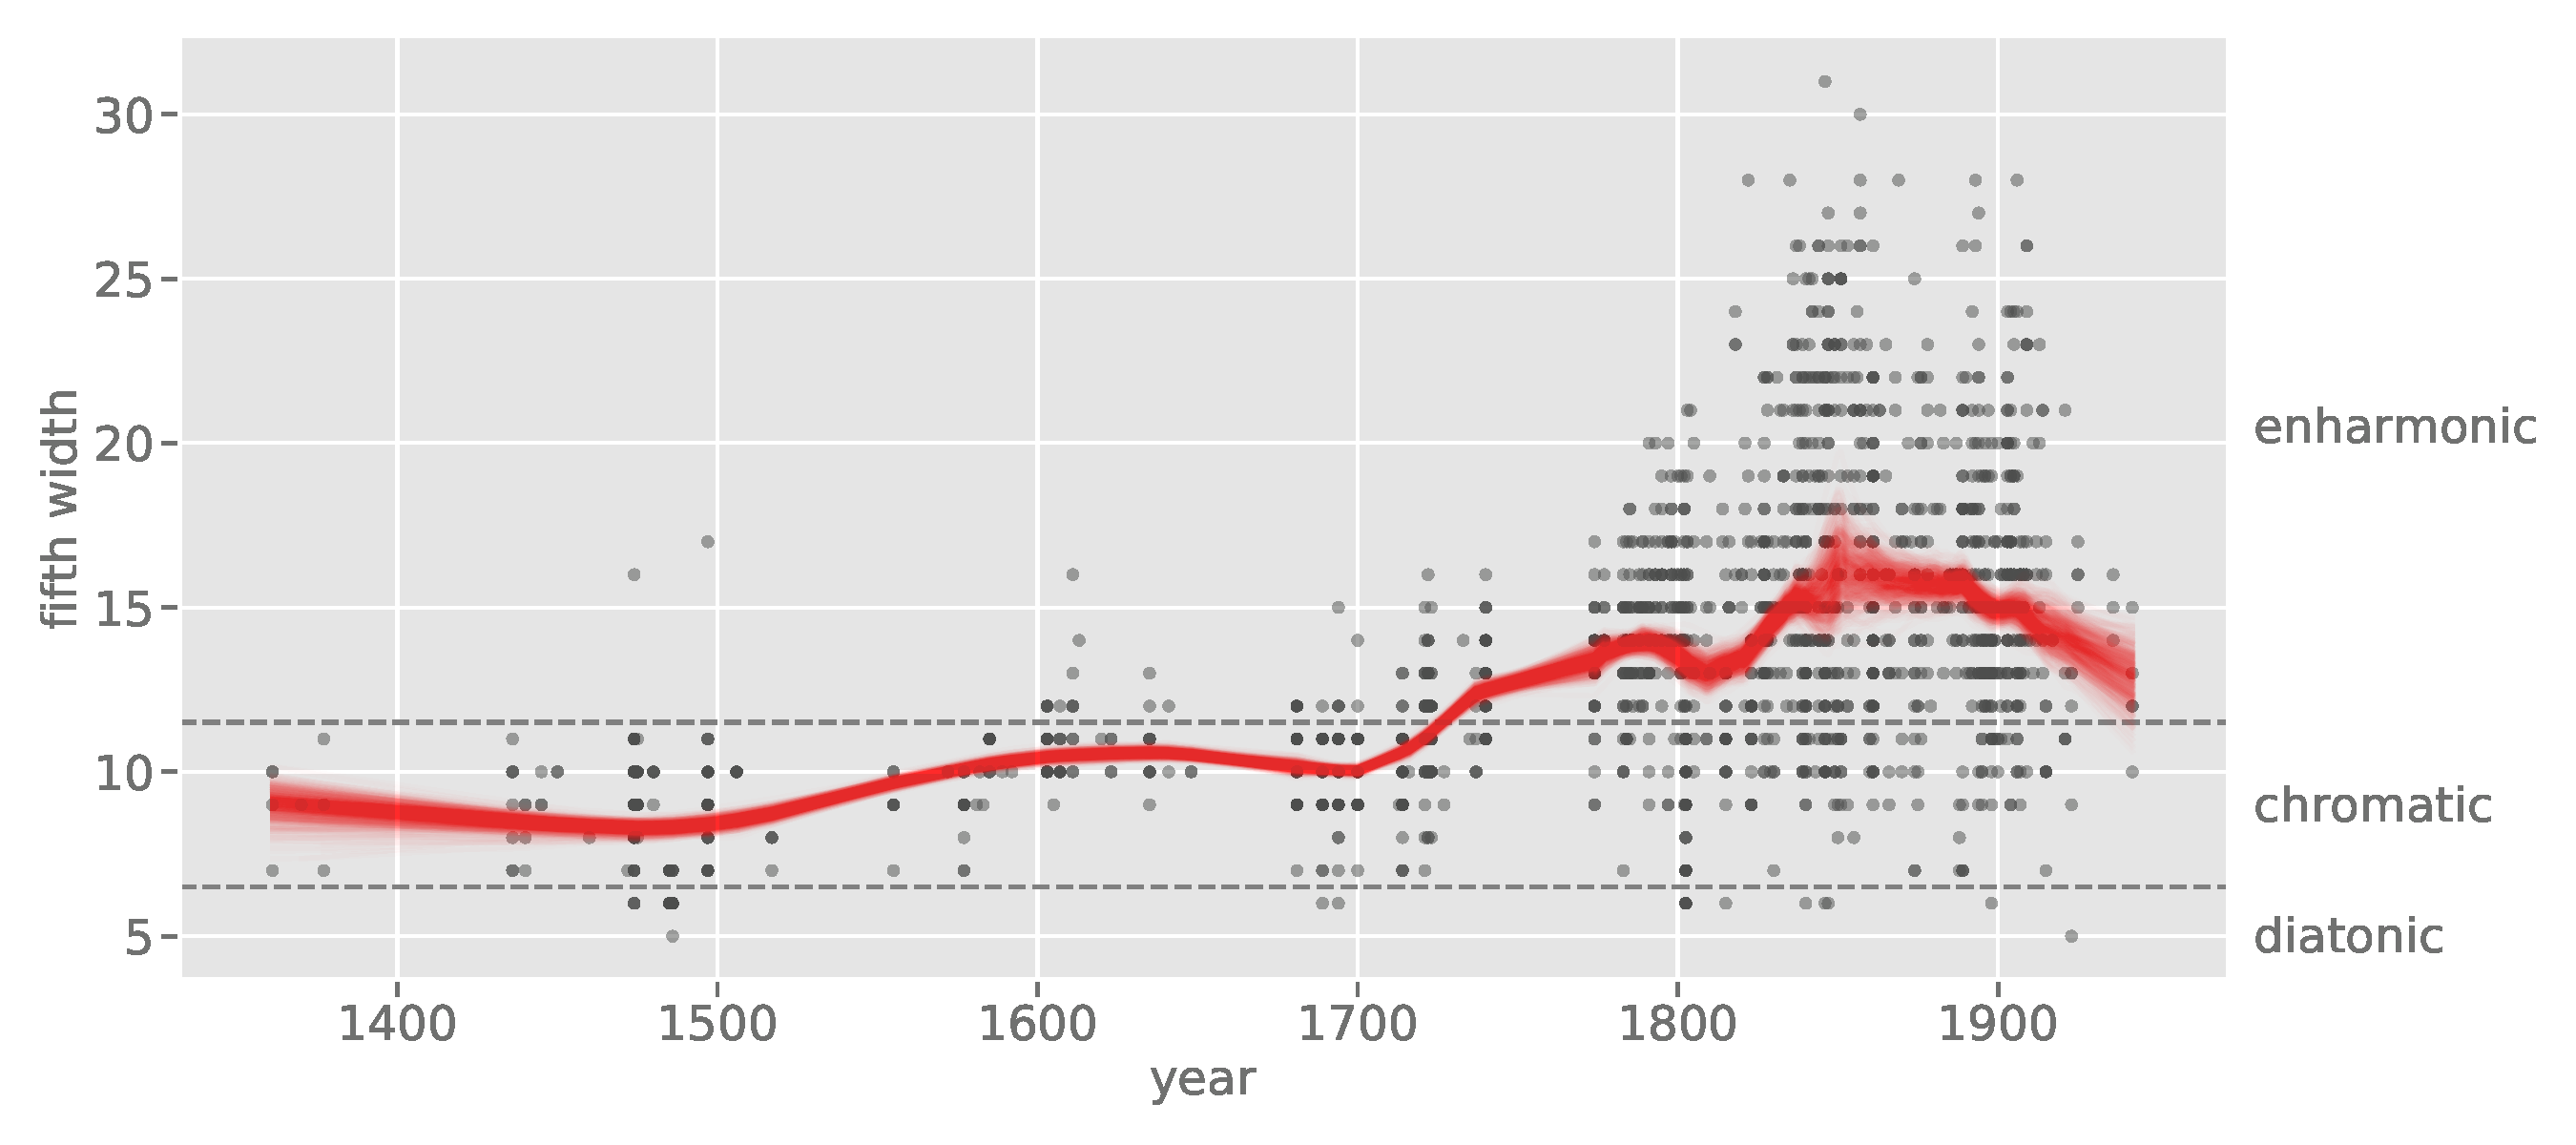
\includegraphics[width=\textwidth]{img/fifth_width.pdf}
    \caption{Historical expansion of tonal material on line of fifths.}
    \label{}
  \end{figure}
\end{frame}

\note[itemize]{
\item Dufay: F\#\# instead of g
\item Ockeghem: Cb instead of C\#
}

\subsection{2. Modelling pieces on the \emph{Tonnetz}}

\begin{frame}{\insertsectionhead}

  Line of fifths is fundamental and simple model but does not explain everything.
  \pause

  $\Rightarrow$ Extend approach to more advanced \alert{models of tonal space}

  \pause
  % Modeling of tonal space in the 19th century: Hauptmann, v. Oettingen, Hostinský, Riemann

  \begin{figure}
    \centering
    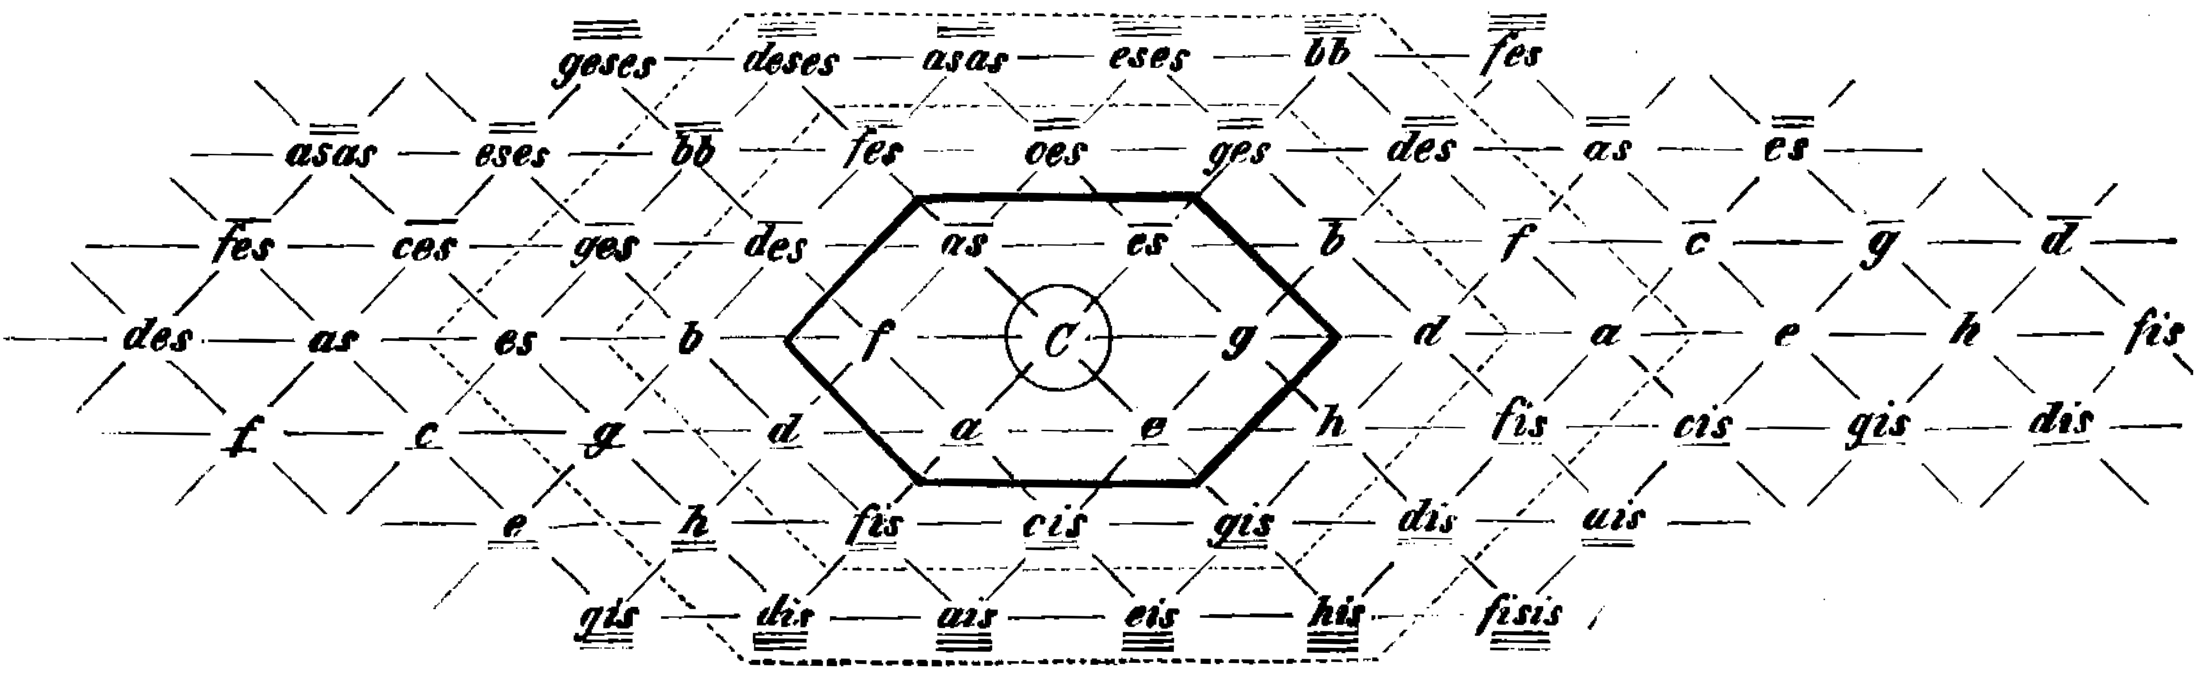
\includegraphics[width=.75\textwidth]{img/hostinsky_tonnetz.png}
    \caption{The \emph{Tonnetz} \citep{Hostinsky1879}.}
    \label{}
  \end{figure}

\end{frame}

\begin{frame}[c]{\insertsectionhead}
  Neo-Riemannian \alert{triadic transformations} on the \emph{Tonnetz}~\citep{Cohn1998}
  \begin{columns}
    \begin{column}{.45\textwidth}
      \begin{itemize}
        \item<2-> \textcolor{epfldark}{parallel ($\mathbf{P}$)}\\ 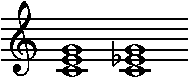
\includegraphics{scores/parallel.pdf}
        \item<3-> \textcolor{canard}{relative ($\mathbf{R}$)}\\ 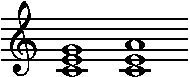
\includegraphics{scores/relative.pdf}
        \item<4-> \textcolor{leman}{leading-tone exchange ($\mathbf{L}$)}\\ 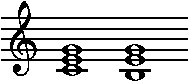
\includegraphics{scores/leading_tone.pdf}
      \end{itemize}

    \end{column}
    %
    \begin{column}{.65\textwidth}
      % TONNETZ WITH ROBERT'S CODE
      %% Figure adapted from https://github.com/DCMLab/TikZ_plot_templates/blob/master/example.tex

  \begin{figure}[c]
    \centering
    % adjust size
    \def\minx{-2}
    \def\maxx{5}
    \def\miny{-2}
    \def\maxy{4}

    % draw hexagons (comment out for not plotting)
    \def\withhex{}
    \newcommand*{\hex}[1]{
      \def\r{0.55}
      \draw[black!7,fill=black!6,visible on=<5->] ($(#1)+(30:\r)$) -- ($(#1)+(90:\r)$) -- ($(#1)+(150:\r)$)  -- ($(#1)+(210:\r)$) -- ($(#1)+(270:\r)$) -- ($(#1)+(330:\r)$) -- cycle;
    }

    \newcommand*{\xy}[2]{
      \pgfmathsetmacro{\x}{#1+cos(60)*#2}
      \pgfmathsetmacro{\y}{sin(60)*#2}
    }
    \newcommand*{\xycoord}[2]{($#1*(1,0)+#2*(60:1)$)}
    \newcommand*{\xycoordcenterbelow}[2]{(${#1+0.333}*(1,0)+{#2+0.333-1}*(60:1)$)}
    \newcommand*{\xycoordcenterabove}[2]{(${#1-0.333}*(1,0)+{#2+0.666}*(60:1)$)}

    \def\r{0.55}
    \tikzstyle{tone}=[circle, draw, fill=white, minimum size=2.5em, thick]
    \scalebox{0.6}{
    \begin{tikzpicture}[scale=2, every path/.style={thick}]
      % create the basic grid
      \foreach \x in {-10,...,10} {
        \foreach \y in {-10,...,10} {
          \pgfmathsetmacro{\xx}{\x+cos(60)*mod(\y+100,2)}
          \pgfmathsetmacro{\yy}{sin(60)*\y}
          \ifthenelse{\x>\minx\AND\x<\maxx\AND\y>\miny\AND\y<\maxy}{
            \ifdefined\withhex\hex{\xx,\yy}\fi
            \coordinate (n_\x_\y) at (\xx,\yy);
            \pgfmathsetmacro{\xMOne}{int(\x-1)}
            \pgfmathsetmacro{\yMOne}{int(\y-1)}
            \pgfmathsetmacro{\yPOne}{int(\y+1)}
            \pgfmathsetmacro{\xxMOne}{\xMOne+cos(60)*mod(\yMOne+100,2)}
            \pgfmathsetmacro{\yyMOne}{sin(60)*\yMOne}
            \pgfmathsetmacro{\yyPOne}{sin(60)*\yPOne}
            \pgfmathsetmacro{\iseven}{int(mod(\y+100,2))}
            \ifthenelse{\xMOne>\minx\AND\xMOne<\maxx}{
              \draw (n_\x_\y) -- (n_\xMOne_\y);
            }{}
            \ifthenelse{\yMOne>\miny\AND\yMOne<\maxy}{
              \draw (n_\x_\y) -- (n_\x_\yMOne);
            }{}
            \ifthenelse{\xMOne>\minx\AND\xMOne<\maxx\AND\yMOne>\miny\AND\yMOne<\maxy}{
              \ifthenelse{\iseven=0}{
                \draw (n_\x_\y) -- (n_\xMOne_\yMOne);
              }{}
            }{}
            \ifthenelse{\xMOne>\minx\AND\xMOne<\maxx\AND\yPOne>\miny\AND\yPOne<\maxy}{
              \ifthenelse{\iseven=0}{
                \draw (n_\x_\y) -- (n_\xMOne_\yPOne);
              }{}
            }{}
          }{}
        }
      }
      % coloured areas
      % \draw[fill=epflred, opacity=0.3] \xycoord{0}{0} -- \xycoord{2}{0} -- \xycoord{2}{1} -- \xycoord{0}{1} -- cycle;
      \draw[fill=epflred, opacity=0.4,visible on=<1->] \xycoord{0}{0} -- \xycoord{1}{0} -- \xycoord{0}{1} -- cycle; % C major
      \draw[fill=epflred, opacity=0.2,visible on=<2->] \xycoord{0}{0} -- \xycoord{1}{0} -- \xycoord{1}{-1} -- cycle; % C minor
      \draw[fill=epflred, opacity=0.2,visible on=<3->] \xycoord{0}{0} -- \xycoord{0}{1} -- \xycoord{-1}{1} -- cycle; % A minor
      \draw[fill=epflred, opacity=0.2,visible on=<4->] \xycoord{1}{0} -- \xycoord{1}{1} -- \xycoord{0}{1} -- cycle; % E minor


      % create tone names
      \foreach \nodename\name/\fifths/\thirds in {
        A+/{A$\sharp$}/-2/3, E+/{E$\sharp$}/-1/3, B+/{B$\sharp$}/0/3, F++/{F$\sharp\sharp$}/1/3, C++/{C$\sharp\sharp$}/2/3, G++/{G$\sharp\sharp$}/3/3,
        F+/{F$\sharp$}/-2/2, C+/{C$\sharp$}/-1/2, G+/{G$\sharp$}/0/2, D+/{D$\sharp$}/1/2, A+/{A$\sharp$}/2/2, E+/{E$\sharp$}/3/2,
        A/A/-1/1, E/E/0/1, B/B/1/1, F+/{F$\sharp$}/2/1, C+/{C$\sharp$}/3/1, G+/{G$\sharp$}/4/1,
        F/F/-1/0, C/C/0/0, G/G/1/0, D/D/2/0, A/A/3/0, E/E/4/0,
        A-/{A$\flat$}/0/-1, E-/{E$\flat$}/1/-1, B-/{B$\flat$}/2/-1, F/F/3/-1, C/C/4/-1, G/G/5/-1
      } {
        \node[tone] (\nodename) at \xycoord{\fifths}{\thirds} {\name};
      }
      % draw some arrows
      % \draw[->, >=stealth, shorten >= 1.5em, shorten <= 1.5em, line width=3pt, epflred] \xycoord{0}{0} -- \xycoord{1}{1};
      % \draw[->, >=stealth, line width=3pt, violet] \xycoordcenterbelow{1}{1} -- \xycoordcenterabove{3}{0};
      % \draw[->, >=stealth, line width=3pt, green] \xycoord{0.5}{1.5} -- \xycoord{1.5}{1.5};
      % \draw[->, >=stealth, line width=3pt, blue] \xycoord{-0.75}{2.5} -- \xycoord{1.25}{2.5};
      \draw[->, >=stealth, line width=2pt, epfldark,visible on=<2->] \xycoordcenterbelow{0}{1} -- \xycoordcenterabove{1}{-1} node [pos=.25, right] {$\mathbf{P}$}; % parallel
      \draw[->, >=stealth, line width=2pt, canard,visible on=<3->] \xycoordcenterbelow{0}{1} -- \xycoordcenterabove{0}{0} node [pos=.3, below] {$\mathbf{R}$}; % relative
      \draw[->, >=stealth, line width=2pt, leman,visible on=<4->] \xycoordcenterbelow{0}{1} -- \xycoordcenterabove{1}{0} node [pos=.2, above] {$\mathbf{L}$}; % leading-tone
    \end{tikzpicture}
    }
    \caption{The \emph{Tonnetz}.}
\end{figure}

    \end{column}
  \end{columns}
\end{frame}

\note[itemize]{
\small
\item While Neo-Riemannian transformations on the \emph{Tonnetz} are a useful analytical
  technique for a great deal of music, it has an obvious limitation:
\item It requires that the music under consideration is triadic.
\item There are a number of approaches trying to extend the classical paradigm, e.g.
  by also considering seventh chords.
\item But as an analyst, one can not know in advance which kinds of sonorities one will
  encounter with a new, maybe unknown piece.
\item Fortunately, there is a way out of this dilemma.
\item We can consider the \emph{Dual Tonnetz} in which not triads but the notes are in the focus.
\item This hexagonal reprentation allows us to visualise notes as they occur in a piece or in a section thereof,
  and to compare pieces with one another.
\item This approach is particularly relevant since we want to understand the historical development of tonality.
}

\begin{frame}[fragile]{\insertsectionhead}

  \begin{columns}
    \begin{column}{.5\linewidth}
      % The \emph{dual Tonnetz}

      \begin{itemize}
        \item<2-> \alert{diatonic} $\pm$ P5\\
        \vspace{1em}
          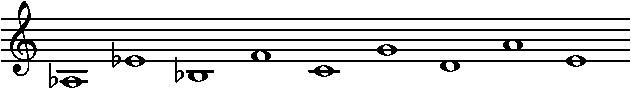
\includegraphics[width=\linewidth]{scores/diatonic.pdf}
        \item<3-> \alert{octatonic} $\pm$ m3, $\pm$ P5\\
        \vspace{1em}
          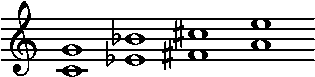
\includegraphics[width=.55\linewidth]{scores/octatonic.pdf}
        \item<4-> \alert{hexatonic} $\pm$ M3, $\pm$ P5\\
        \vspace{1em}
          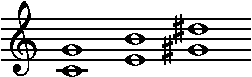
\includegraphics[width=.45\linewidth]{scores/hexatonic.pdf}
      \end{itemize}
    \end{column}
    %
    \begin{column}{.5\linewidth}

    \begin{figure}[tbp]
    \centering
    \newcommand*{\hex}[1]{
      \def\r{0.55}
      \draw[black!6,fill=black!4] ($(#1)+(30:\r)$) -- ($(#1)+(90:\r)$) -- ($(#1)+(150:\r)$)  -- ($(#1)+(210:\r)$) -- ($(#1)+(270:\r)$) -- ($(#1)+(330:\r)$) -- cycle;
    }
    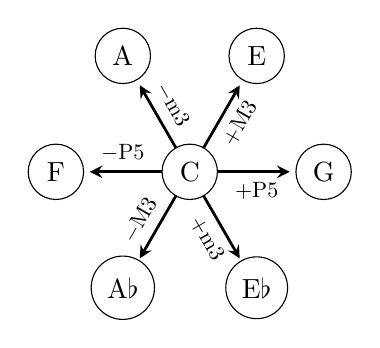
\begin{tikzpicture}[scale=1.7]
      % hexagon
      \hex{0,0}
      % notes
      \foreach \a/\l/\i/\p in {
        0/G/{$+$P5}/below,
        -60/{E$\flat$}/{$+$m3}/below,
        -120/{A$\flat$}/{$-$M3}/above,
        -180/F/{$-$P5}/above,
        -240/A/{$-$m3}/above,
        -300/E/{$+$M3}/below,
        1000/// % hack to avoid weird tikz label problem
      } {
        \ifthenelse{\a=1000}{}{
          \hex{\a:1}
          \draw (\a:0.15) edge[->,>=stealth,line width=1,shorten >=.5em] node[\p ,sloped,fill=white,fill opacity=0,text opacity=1] {\scalebox{0.8}{\i}} (\a:0.85);
          \node [circle,draw,black, fill=white, minimum size=2em] at (\a:1) {\l};
        }
      }
      % center
      \node [circle,draw,black, fill=white, minimum size=2em] at (0,0) {C};
    \end{tikzpicture}
    % \caption{Primary intervals with respect to C.}\label{fig:primary_intervals}
  \end{figure}
\end{column}
\end{columns}
\end{frame}

\begin{frame}{\insertsectionhead}

  \begin{columns}
    \begin{column}{.33\linewidth}
      \centering
      \alert{diatonic}

      \vspace{1em}

      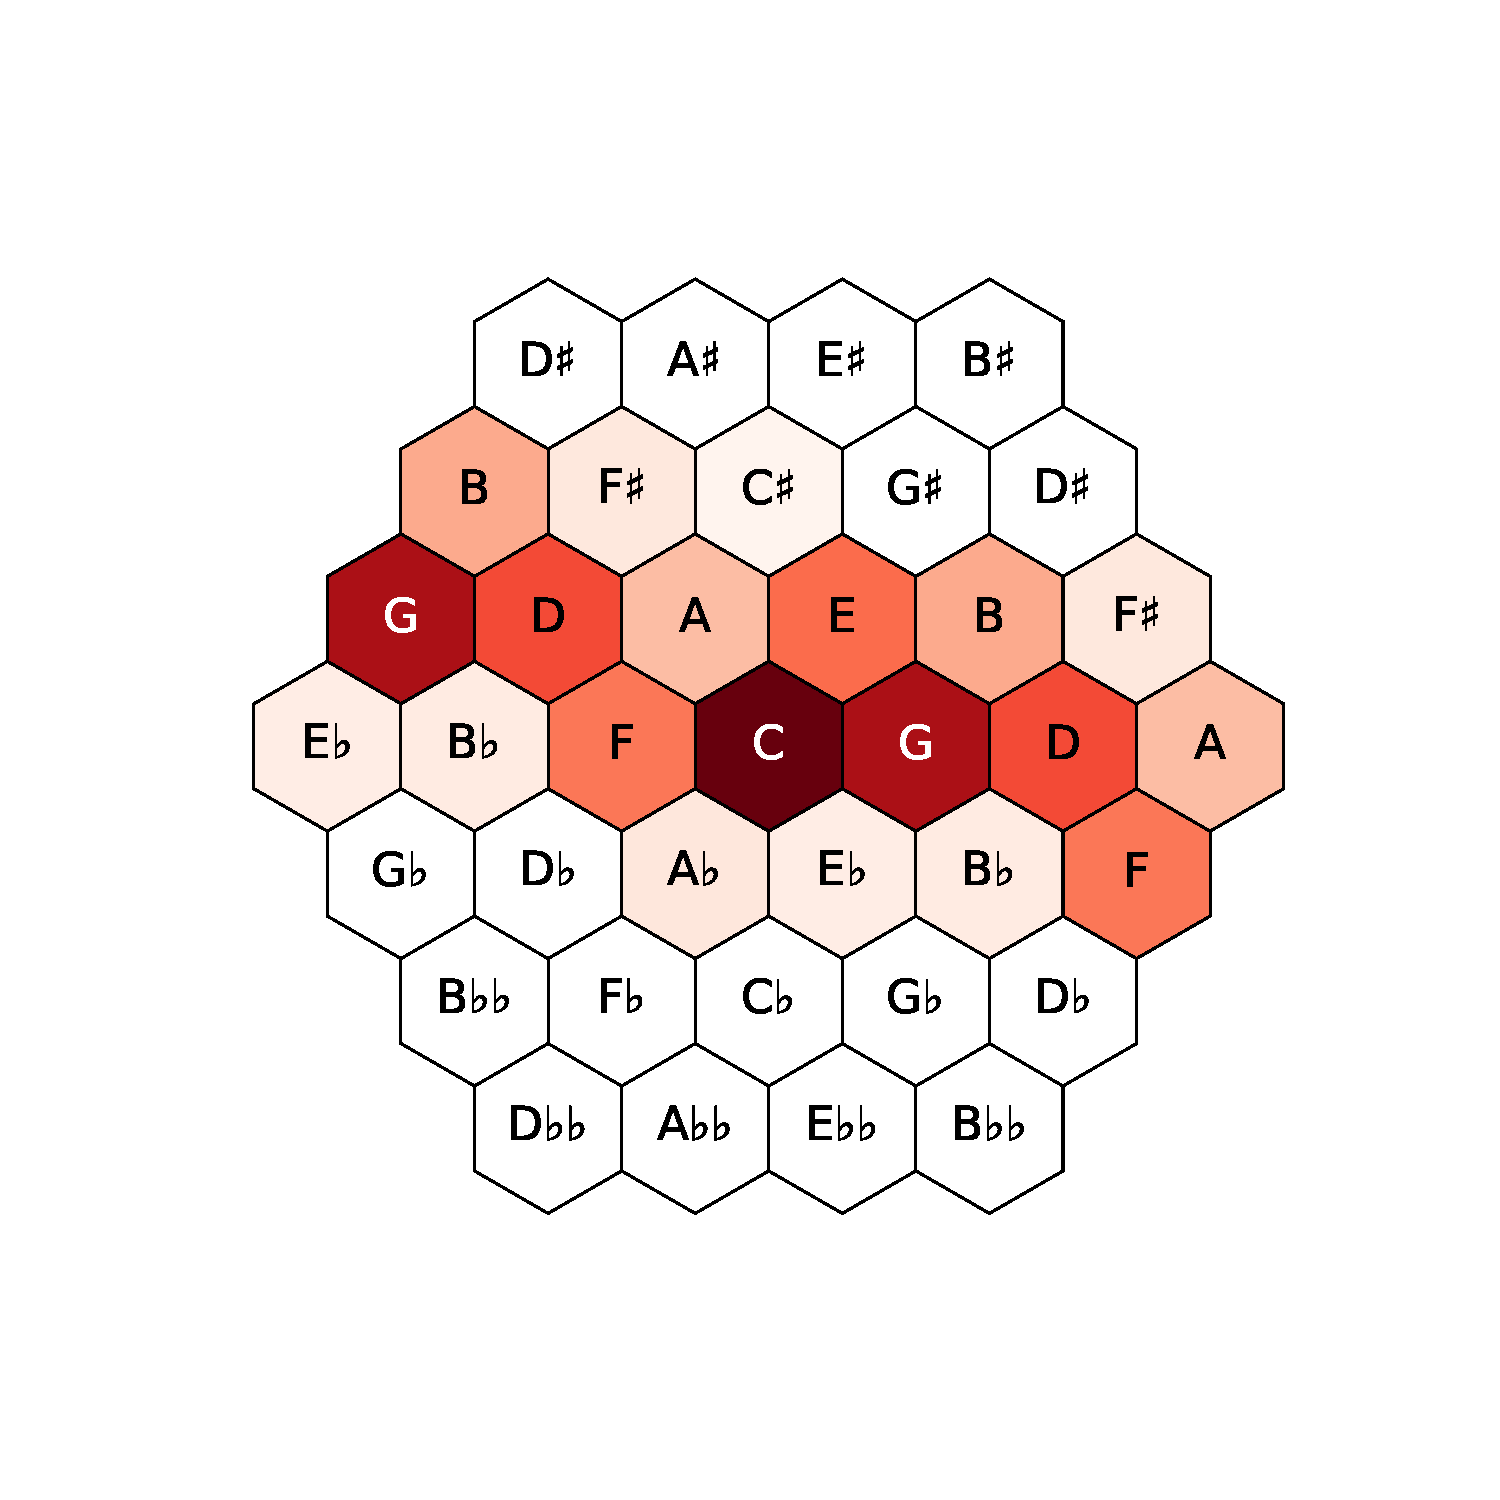
\includegraphics[trim=0 100 0 100, clip, width=\linewidth]{img/bach.pdf}
      Bach, \emph{Prelude in C major}, BWV~846 (1722).
    \end{column}
    %
    \pause
    %
    \begin{column}{.33\linewidth}
      \centering
      \alert{hexatonic}

      \vspace{1em}

      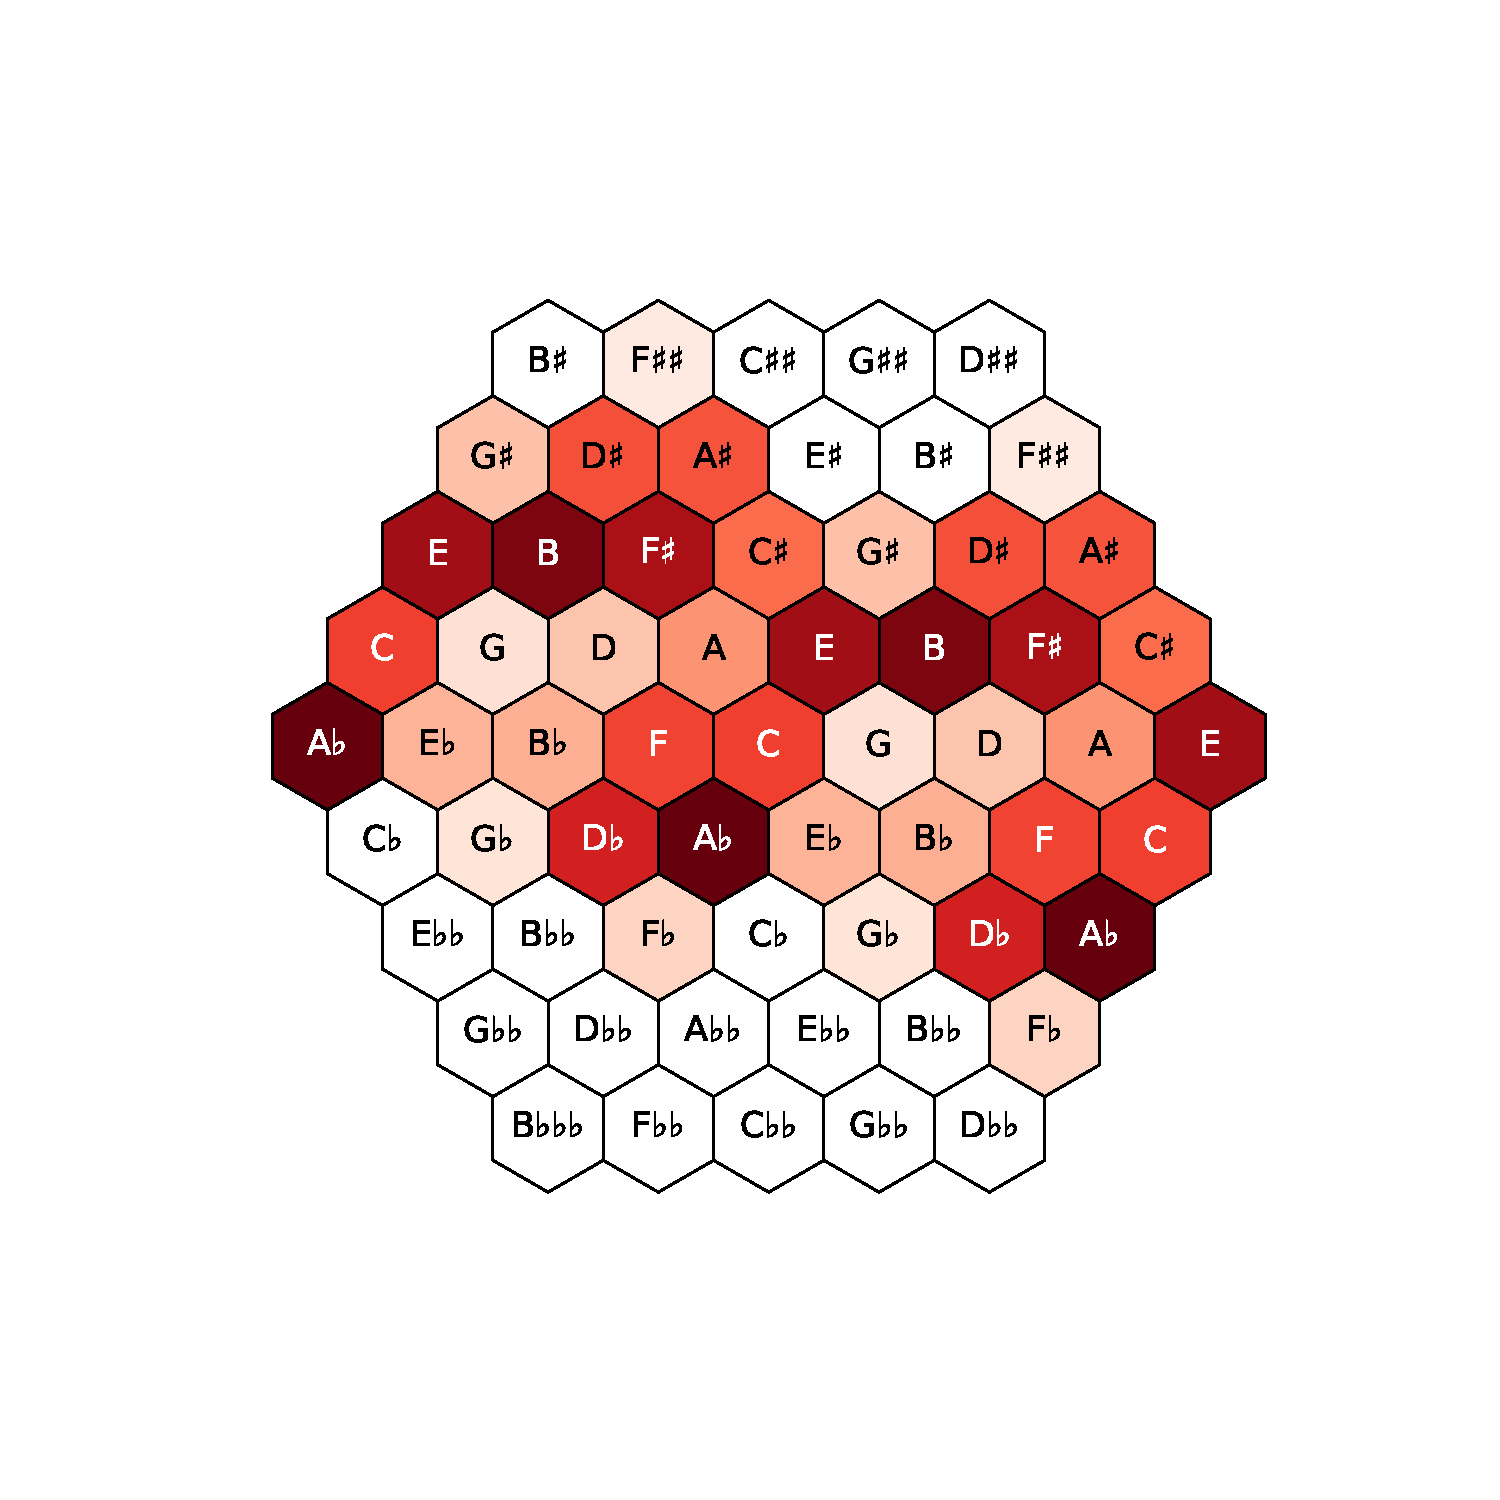
\includegraphics[trim=0 100 0 100, clip, width=\linewidth]{img/liszt.pdf}
      Liszt, \emph{Lugubre gondola I}, S.~200/1~(1882).
    \end{column}
    %
    \pause
    %
    \begin{column}{.33\linewidth}
      \centering
      \alert{octatonic}

      \vspace{1em}

      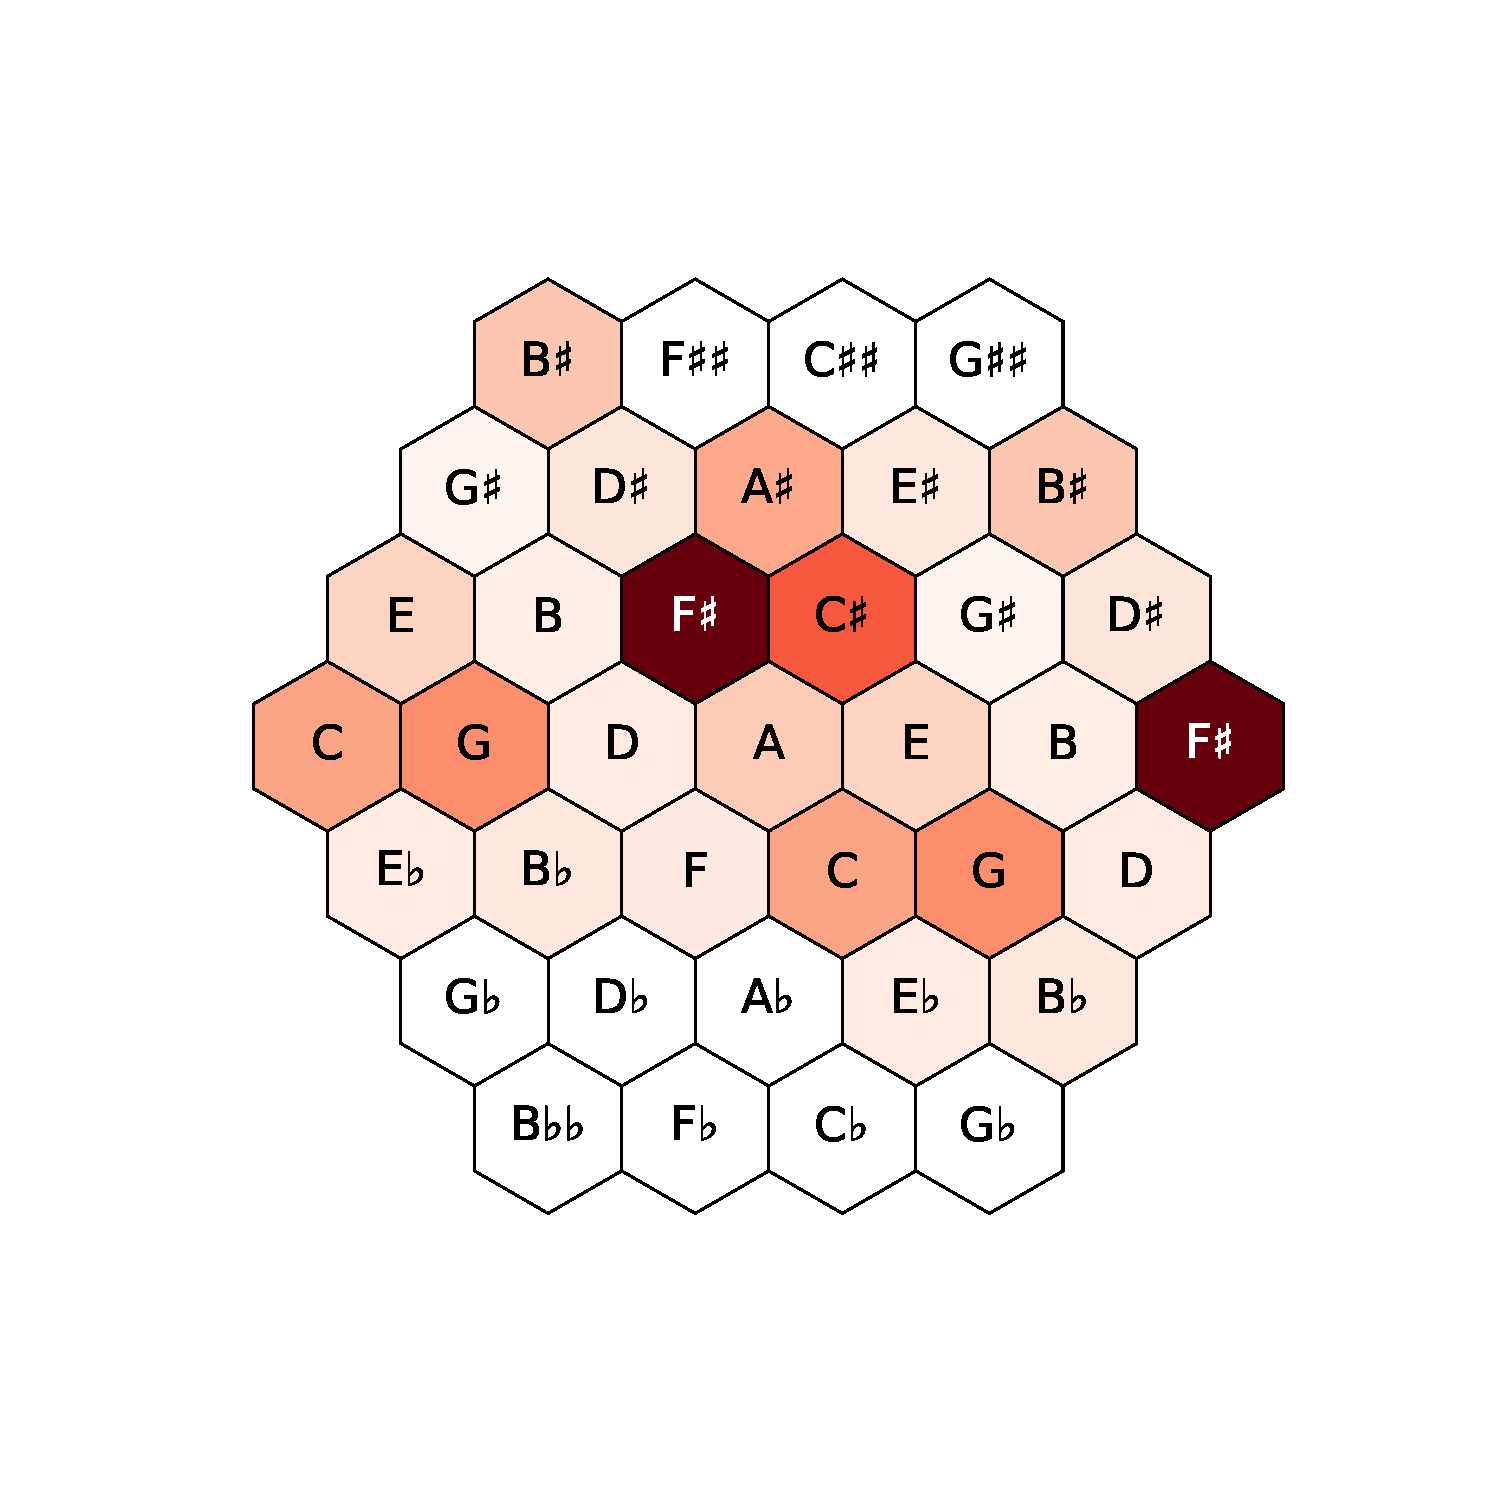
\includegraphics[trim=0 130 0 100, clip, width=\linewidth]{img/scriabin.pdf}
      Scriabin, \emph{Prelude}, op.~74/2~(1914).
    \end{column}
  \end{columns}

  % \begin{figure}
  %   \centering
  %   \begin{subfigure}[t]{.3\textwidth}
  %     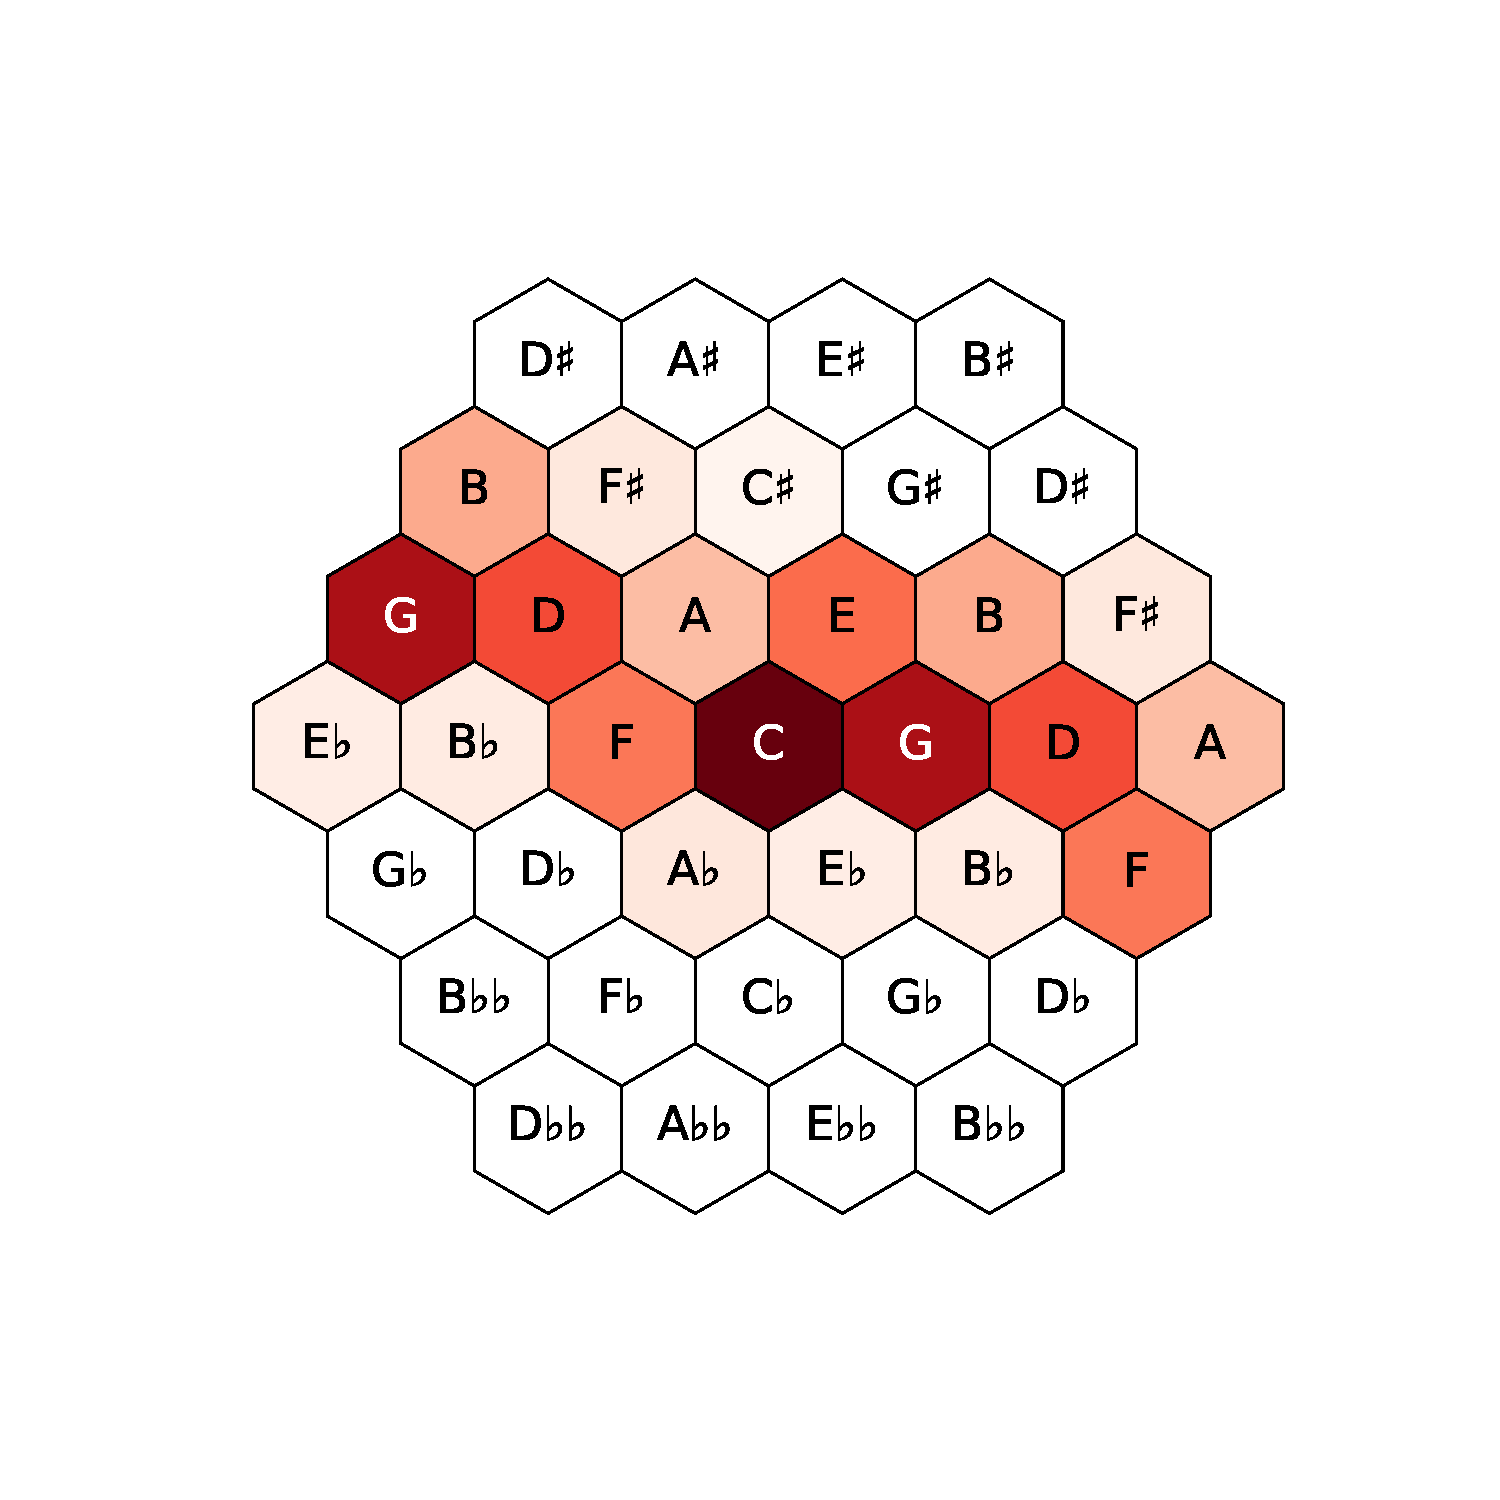
\includegraphics[width=\linewidth]{img/bach.pdf}
  %     \subcaption*{Bach, \emph{Prelude in C major}, WTC I, (1722).}
  %   \end{subfigure}
  %   \hfill
  %   \begin{subfigure}[t]{.3\textwidth}
  %
  %   \end{subfigure}
  %   \hfill
  %   \begin{subfigure}[t]{.3\textwidth}
  %
  %   \end{subfigure}
  %   \caption{Historical differences in note distributions.}
  % \end{figure}
\end{frame}

\note[itemize]{
\item Most importantly, this approach does not need a reduction to triads prior to analysis, since the notes can
  be taken from the score as they are written.
\item However, as in the case of the classical \emph{Tonnetz}, we consider octave related notes as equivalent.
}

\begin{frame}{\insertsectionhead}
  Computational model assumptions
  \begin{enumerate}[\color{epflred}1.]
    \item all notes are related to a \alert{tonal center}
    \item relations are given by (combinations of) \alert{intervals} on the \emph{Tonnetz}
  \end{enumerate}
\end{frame}

\begin{frame}{\insertsectionhead}
  \begin{enumerate}[\color{epflred}1.]
    \item \textbf{Initial computational model and analysis}\\\citet{Moss2019a}.~\citetitle{Moss2019a}.
    \item \textbf{Extensions of model}\\\citet{Lieck2020}.~\citetitle{Lieck2020}.
    \item \textbf{Extensions of analysis}\\\citet{Moss2020b}.~\citetitle{Moss2020b}.
  \end{enumerate}
\end{frame}


\begin{frame}{\insertsectionhead}

  \begin{figure}[h]
    \onslide<1->{
	\begin{subfigure}{0.44\linewidth}
		\centering
		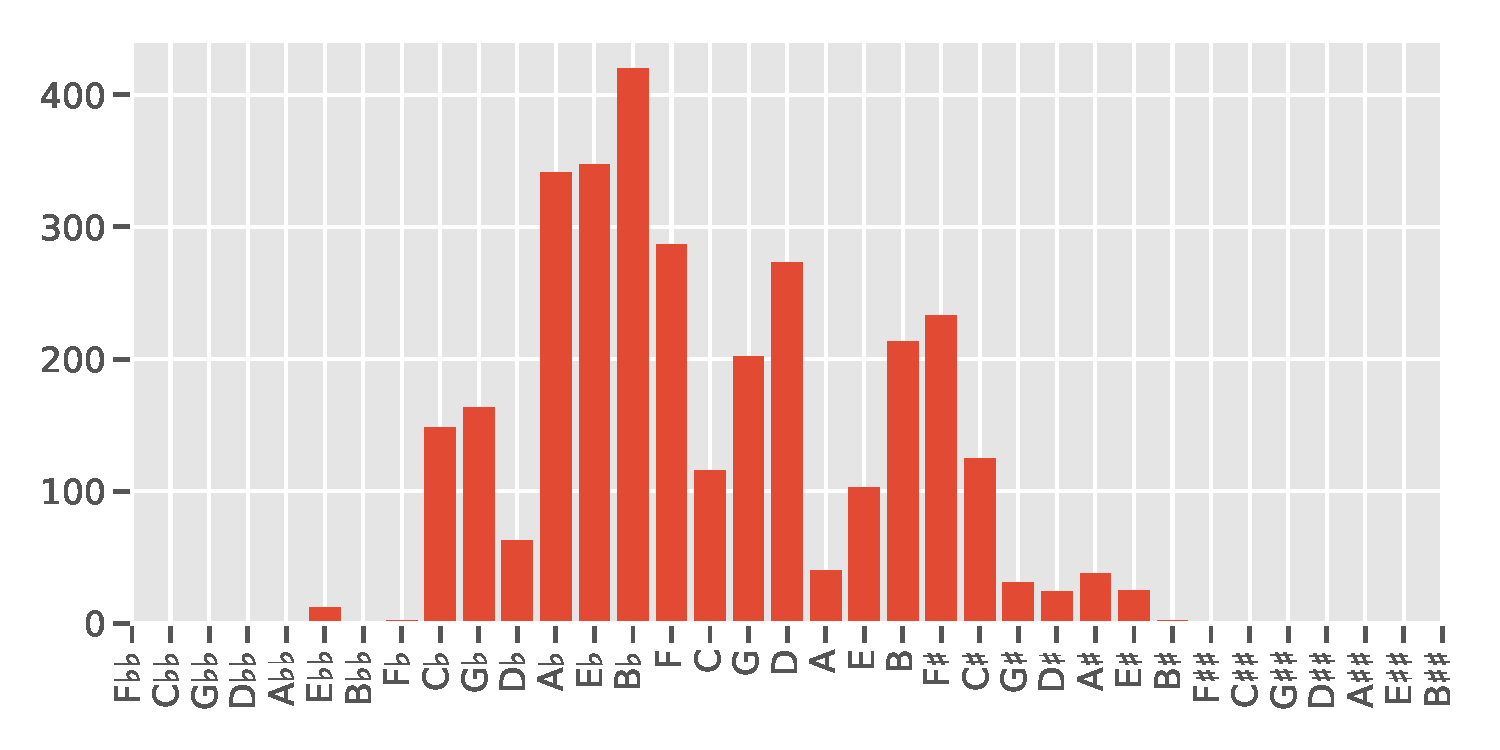
\includegraphics[width=\textwidth]{img/tpc_dists.pdf}
	\end{subfigure}}
  %
  \hfill
  \onslide<2->{
	\begin{subfigure}{0.24\linewidth}
		\centering
		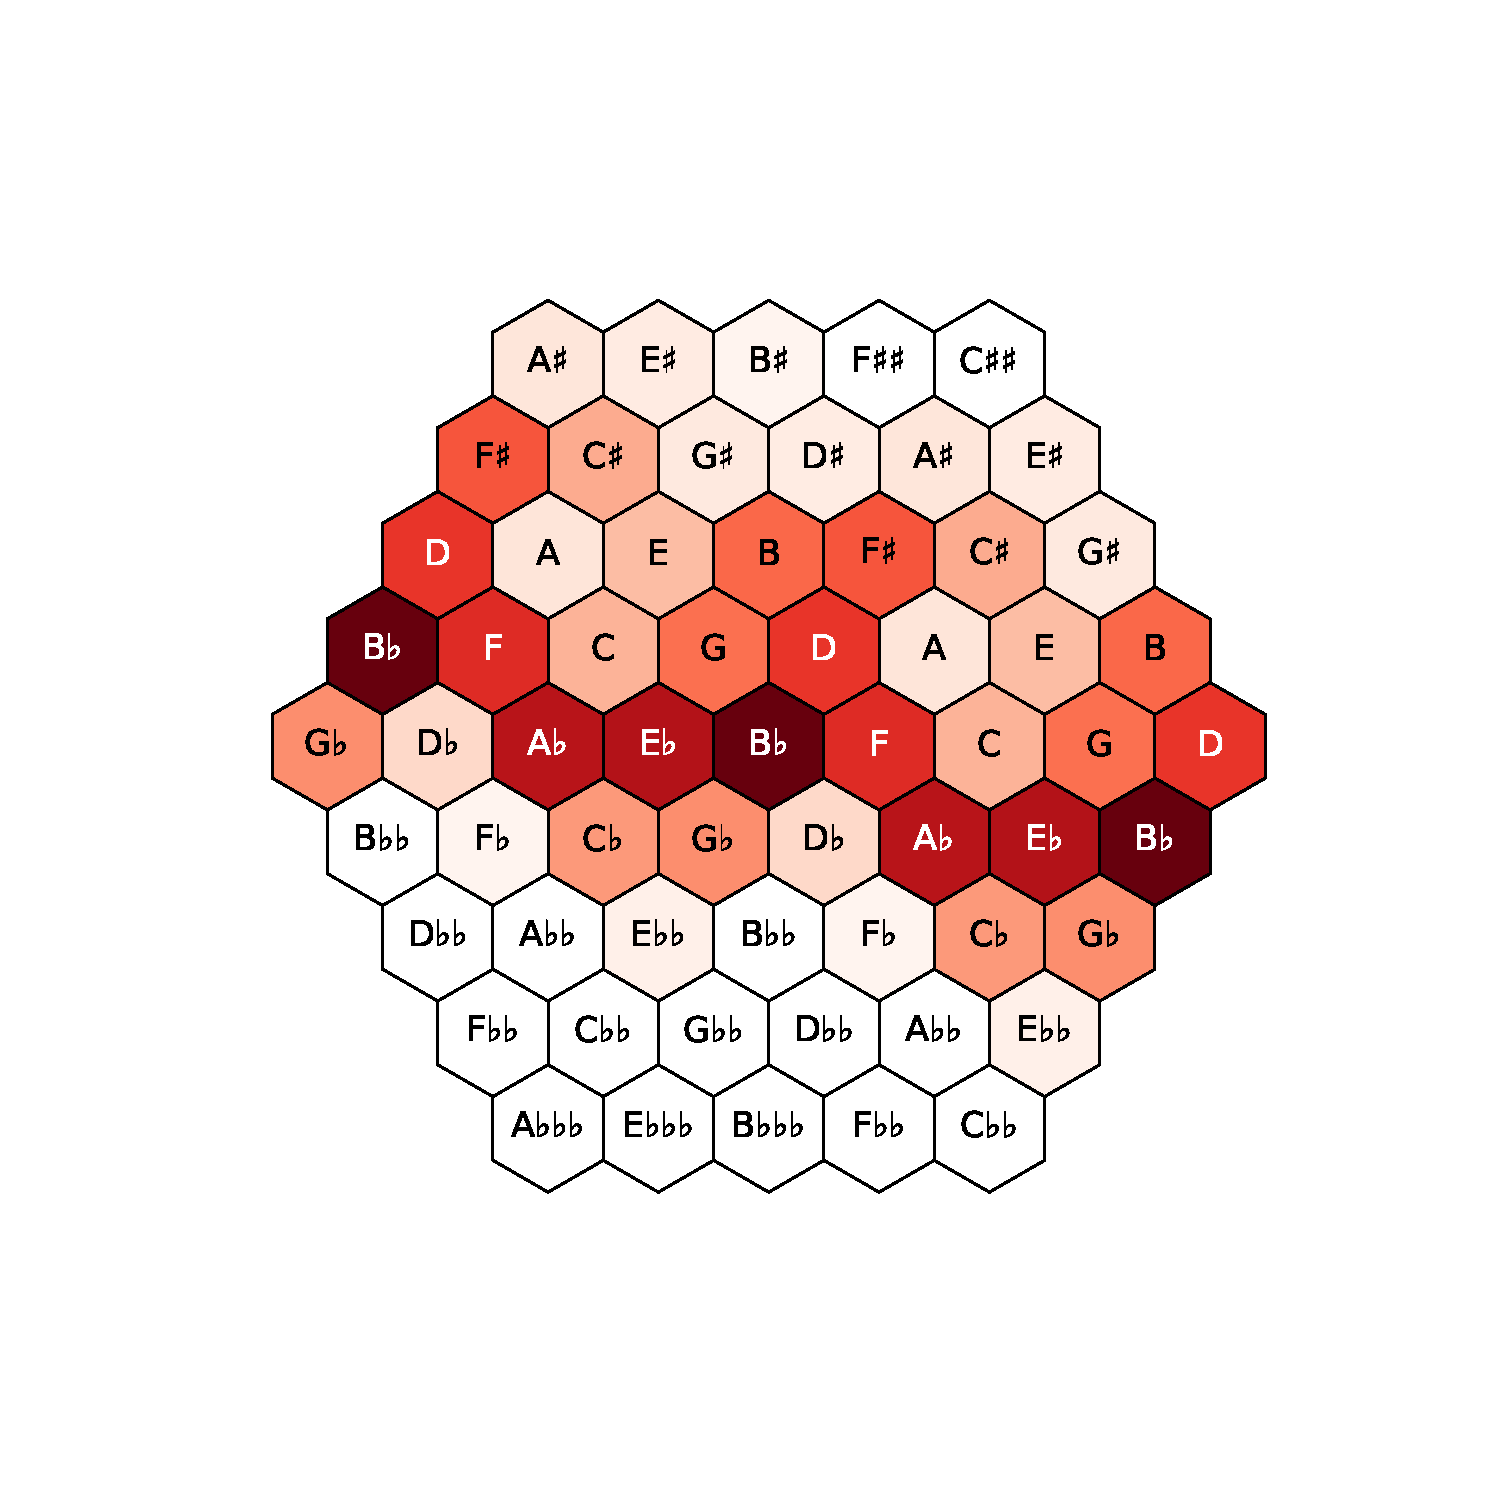
\includegraphics[width=\textwidth, trim=110 140 110 140,clip]{img/Schubert_90_2.pdf}
	\end{subfigure}}
  %
  \hfill
  \onslide<3->{
  \begin{subfigure}{0.29\linewidth}
		\centering
		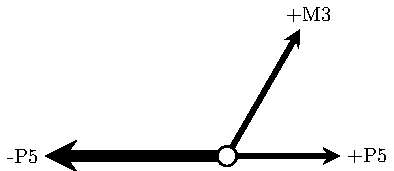
\includegraphics[width=\textwidth]{img/tikz_Schubert_90_2.pdf}
	\end{subfigure}}
	\caption{F. Schubert, \emph{Impromptu}, op. 90/2 in E$\flat$ major.}
	% \label{}
\end{figure}

\onslide<4->{

Model finds six \alert{interval parameters} that best explain the notes in a piece.
\begin{itemize}
  \item only based on \alert{explicit} music-theoretical assumptions $\rightarrow$ criticism
  \item looking at all parameters for all pieces in the corpus shows \alert{historical trends}
\end{itemize}
}

\end{frame}

\begin{frame}
  % \begin{columns}
  %   \begin{column}{.4\textwidth}
  %     \begin{itemize}
  %       \item Computational Model to infer most likely interval usage~\citep{Lieck2020}
  %       \item Perfect fifths are highly relevant throughout history
  %       \item Major and minor third directions are explored abundantly in the 19th century
  %     \end{itemize}
  %   \end{column}
  %   %
  %   \begin{column}{.6\textwidth}
      \begin{figure}
        \centering
        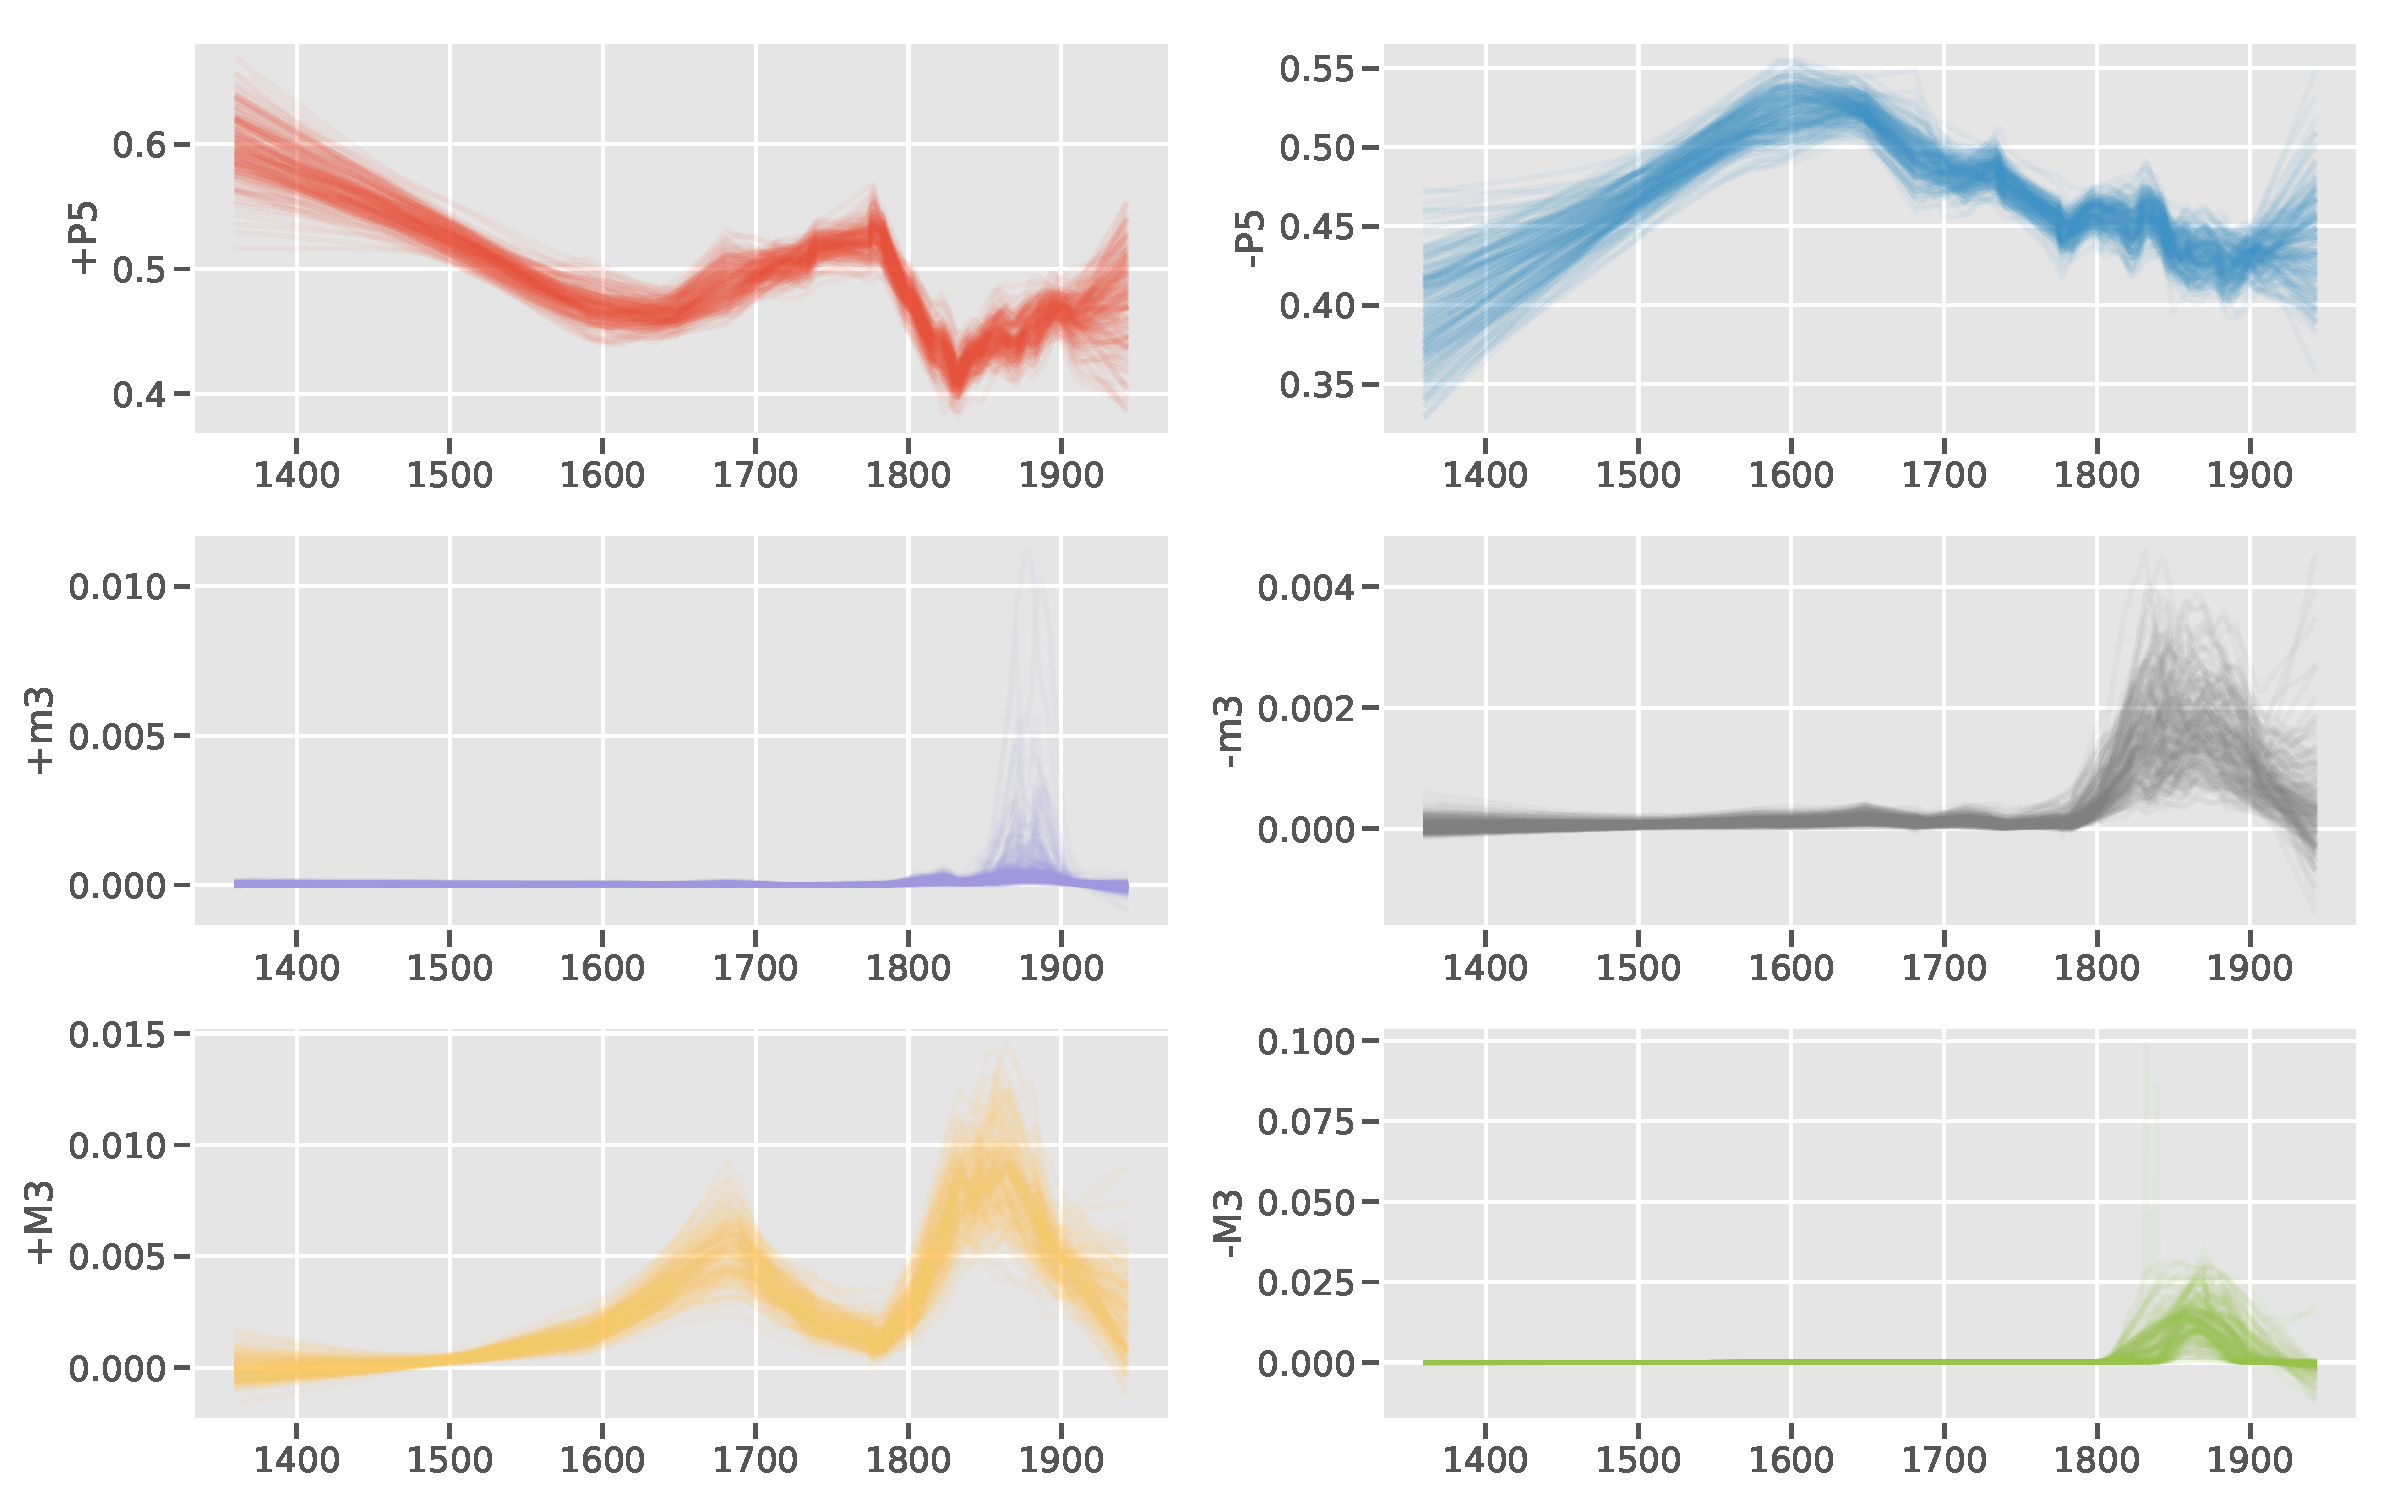
\includegraphics[width=.65\textwidth]{img/bootstrapped_weights.pdf}
        \caption{Historical changes in interval usage on the \emph{Tonnetz}.}
        \label{}
      \end{figure}
  %   \end{column}
  % \end{columns}
\end{frame}

% \begin{frame}{\insertsectionhead}
%   \begin{enumerate}[\color{epflred}1.]
%     \item<1-> model finds \alert{best explanations} for relations between notes
%     \item<2-> only based on \alert{explicit assumptions} of the model $\rightarrow$ criticism
%     \item<3-> corpus studies allow to analyze \alert{changes of tonality} on a large scale
%   \end{enumerate}
% \end{frame}

% \begin{frame}{Summary and Prospects}
%   \begin{enumerate}[\color{epflred}1.]
%     \item \ldots
%     \item \ldots
%     \item Tonality tells only one part of the story. Many other aspects of music are relevant as well,
%     e.g. form, meter, instrumentation, tuning, social contexts, reception, \ldots
%   \end{enumerate}
% \end{frame}

% \section{Summary and Conclusion}

\begin{frame}{Summary}
  \begin{enumerate}[\color{epflred}1.]
  \item<+-> a small set of chords is shared by many composers
  \item<+-> this core makes up large portions of their harmonic language
  \item<+-> important aspects of chord distributions are not yet well-understood
  \item<+-> the line of fifths can be retrieved from data
  \item<+-> using the \emph{Tonnetz} reveals stylistic differences
  \item<+-> both can be expanded from the study of single pieces to entire repertoires
\end{enumerate}
\end{frame}

\begin{frame}{Conclusion}
  \textbf{Computational Music Analysis}
  \begin{enumerate}[\color{epflred}1.]\pause
    \item<+-> forces precise definitions and models
    \item<+-> allows to test music theoretical concepts on large corpora
    \item<+-> facilitates interactions with other areas within and beyond musicology
    \item<+-> requires reflection, critique, and interpretation
  \end{enumerate}
\end{frame}

% \againframe<8->{disciplines}

% \begin{frame}{}
%   \begin{figure}
%     \centering
%     
\includegraphics[height=.9\textheight]{img/dcml.jpg}
%     \caption*{Digital and Cognitive Musicology Lab, Lausanne, 2019}
%   \end{figure}
% \end{frame}

\begin{frame}[standout]
  Thank you very much!
\end{frame}


%%% BACKMATTER %%%

\appendix

\begin{frame}[allowframebreaks]
  \renewcommand*{\bibfont}{\footnotesize}
  \printbibliography
\end{frame}

\end{document}
